\chapter{Estimation of Required Number of Samples}
\label{sec:statistics}
\section{Brute Force Estimation}
\label{sec:Brute}

First an estimate for the number of samples needed to achieve different confidence level and intervals is investigated. The number of samples needed is found using the normal approximation of the Binomial proportion \citep{SampleNumURC}. 

\begin{equation}\label{eq:numSamples}
\frac{z_{\frac{\alpha}{2}} \sqrt{\frac{\hat{\gamma}\left(1-\hat{\gamma}\right)}{N}}}{\hat{\gamma}} < m
\end{equation} 
\begin{where}
\va{$z_{\frac{\alpha}{2}}$}{is the $100(1-\frac{\alpha}{2})$-th percentile of the standard normal distribution}{1}
\va{$\hat{\gamma}$}{is the estimated probability}{1}
\va{N}{is the number of samples}{1}
\va{m}{is the margin around $\hat{\gamma}$}{1}
\end{where}

From the \autoref{chap:introduction} the value of $\hat{\gamma}$ is set to $10^{-5}$. With that estimations of the number of samples needed to uphold different confidence level and intervals can be found as seen in \autoref{tab:numSample}. 

\begin{table}[H]
\centering
\begin{tabular}{c|l|l|l|l|l|l|}
\multicolumn{2}{l}{}  & \multicolumn{5}{c}{\textbf{Confidence level}} \\ \cline{3-7} 
\multicolumn{2}{l|}{}  & \textbf{80 \%} & \textbf{85 \%} & \textbf{90 \%} & \textbf{95 \%} & \textbf{99 \%} \\ \cline{2-7} 
\multirow{5}{*}{{\rotatebox{90}{\textbf{Interval}}}} & \textbf{$\pm$0.5 dB} & 11.0E+6 & 13.9E+6 & 18.2E+6 & 25.8E+6 & 44.6E+6 \\ \cline{2-7} 
 & \textbf{$\pm$1 dB} 	& 2.45E+6 	& 3.09E+6 	& 4.04E+6 	& 5.73E+6 	& 9.90E+6 \\ \cline{2-7} 
 & \textbf{$\pm$1.5 dB} & 965E+3 	& 1.22E+6 	& 1.59E+6 	& 2.26E+6 	& 3.90E+6 \\ \cline{2-7} 
 & \textbf{$\pm$2 dB} 	& 480E+3 	& 606E+3 	& 791E+3 	& 1.12E+6 	& 1.94E+6 \\ \cline{2-7} 
 & \textbf{$\pm$2.5 dB} & 271E+3 	& 342E+3 	& 447E+3 	& 634E+3 	& 1.10E+6 \\ \cline{2-7} 
\end{tabular}
\caption{Estimated number of samples for different confidence levels and intervals.}
\label{tab:numSample}
\end{table}

\newpage
\subsection{Statistics method for rare events}\label{sampleEQ}
As seen in \autoref{tab:numSample}, there is a need of a high number of samples, to get a high confidence interval. The reason for this, is the need for a high number of rare events to occur to get a high confidence interval for these events. 

For simulation purposes there have been developed some methods to handle this problem. One of them is importance sampling. Importance sampling changes the distribution where the samples is taken from. By changing the distribution, so the rare events is not rare anymore and a high number of them can be samples with a smaller sample population. When introducing this new distribution, an example is given in \autoref{IMD}. There is also introduced a weighting factor, which is defined from the change in the distribution, see \autoref{IMW}. 

\begin{minipage}[t]{0.48\textwidth}
\centering
\begin{figure}[H]
% This file was created by matlab2tikz.
%
%The latest updates can be retrieved from
%  http://www.mathworks.com/matlabcentral/fileexchange/22022-matlab2tikz-matlab2tikz
%where you can also make suggestions and rate matlab2tikz.
%
\definecolor{mycolor1}{rgb}{0.00000,0.44700,0.74100}%
\definecolor{mycolor2}{rgb}{0.85000,0.32500,0.09800}%
%
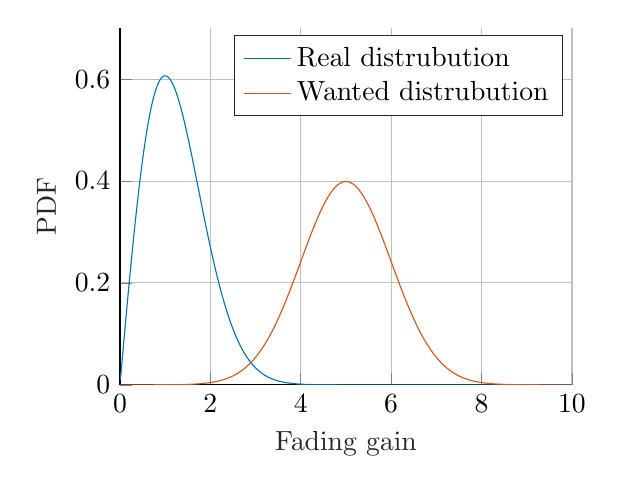
\begin{tikzpicture}

\begin{axis}[%
width=2.260in,
height=1.783in,
at={(0.758in,0.481in)},
scale only axis,
xmin=0,
xmax=10,
xlabel style={font=\color{white!15!black}},
xlabel={Fading gain},
ymin=0,
ymax=0.7,
ylabel style={font=\color{white!15!black}},
ylabel={PDF},
axis background/.style={fill=white},
axis x line*=bottom,
axis y line*=left,
xmajorgrids,
ymajorgrids,
legend style={legend cell align=left, align=left, draw=white!15!black}
]
\addplot [color=mycolor1]
  table[row sep=crcr]{%
0.01	0.00999950001249979\\
0.02	0.0199960003999733\\
0.03	0.0299865030370444\\
0.04	0.0399680127965873\\
0.05	0.0499375390462291\\
0.06	0.0598920971417062\\
0.07	0.0698287099160336\\
0.08	0.0797444091634426\\
0.09	0.0896362371170562\\
0.1	0.0995012479192682\\
0.11	0.109336509083806\\
0.12	0.119139102948458\\
0.13	0.128906128117462\\
0.14	0.138634700892553\\
0.15	0.148321956691685\\
0.16	0.157965051454446\\
0.17	0.167561163033209\\
0.18	0.177107492569052\\
0.19	0.186601265851529\\
0.2	0.196039734661351\\
0.21	0.20542017809507\\
0.22	0.214739903870881\\
0.23	0.223996249614663\\
0.24	0.233186584125389\\
0.25	0.242308308619086\\
0.26	0.2513588579505\\
0.27	0.260335701811684\\
0.28	0.269236345906715\\
0.29	0.278058333101787\\
0.3	0.28679924454993\\
0.31	0.29545670078966\\
0.32	0.304028362816841\\
0.33	0.312511933129105\\
0.34	0.320905156742185\\
0.35	0.32920582217752\\
0.36	0.337411762420564\\
0.37	0.345520855849202\\
0.38	0.35353102713174\\
0.39	0.361440248093947\\
0.4	0.369246538554654\\
0.41	0.376947967129452\\
0.42	0.384542652002031\\
0.43	0.392028761662774\\
0.44	0.399404515614205\\
0.45	0.406668185042938\\
0.46	0.413818093457807\\
0.47	0.420852617293866\\
0.48	0.427770186482008\\
0.49	0.434569284983937\\
0.5	0.441248451292298\\
0.51	0.447806278895774\\
0.52	0.454241416709002\\
0.53	0.460552569467164\\
0.54	0.466738498085176\\
0.55	0.472798019981398\\
0.56	0.478730009365815\\
0.57	0.484533397492695\\
0.58	0.490207172877729\\
0.59	0.495750381479702\\
0.6	0.501162126846763\\
0.61	0.506441570227405\\
0.62	0.511587930646273\\
0.63	0.516600484944962\\
0.64	0.521478567787987\\
0.65	0.526221571634127\\
0.66	0.530828946673393\\
0.67	0.53530020072987\\
0.68	0.539634899130721\\
0.69	0.543832664541672\\
0.7	0.547893176769308\\
0.71	0.551816172530543\\
0.72	0.555601445189659\\
0.73	0.559248844463295\\
0.74	0.562758276093856\\
0.75	0.566129701491755\\
0.76	0.569363137346994\\
0.77	0.57245865521056\\
0.78	0.575416381046157\\
0.79	0.578236494752822\\
0.8	0.580919229658953\\
0.81	0.583464871988351\\
0.82	0.585873760298851\\
0.83	0.588146284894147\\
0.84	0.590282887209454\\
0.85	0.59228405917163\\
0.86	0.594150342534417\\
0.87	0.595882328189485\\
0.88	0.59748065545394\\
0.89	0.598946011335012\\
0.9	0.600279129772627\\
0.91	0.601480790860574\\
0.92	0.602551820047013\\
0.93	0.603493087315054\\
0.94	0.604305506344164\\
0.95	0.604990033653156\\
0.96	0.605547667725531\\
0.97	0.605979448117943\\
0.98	0.60628645455257\\
0.99	0.606469805994172\\
1	0.606530659712633\\
1.01	0.606470210331772\\
1.02	0.606289688865223\\
1.03	0.605990361740194\\
1.04	0.605573529809886\\
1.05	0.60504052735539\\
1.06	0.604392721077861\\
1.07	0.603631509081768\\
1.08	0.602758319850017\\
1.09	0.601774611211763\\
1.1	0.60068186930368\\
1.11	0.599481607525511\\
1.12	0.598175365490659\\
1.13	0.596764707972633\\
1.14	0.595251223848097\\
1.15	0.593636525037321\\
1.16	0.591922245442784\\
1.17	0.590110039886701\\
1.18	0.58820158304821\\
1.19	0.586198568400981\\
1.2	0.584102707151966\\
1.21	0.581915727182025\\
1.22	0.579639371989138\\
1.23	0.577275399634905\\
1.24	0.574825581695038\\
1.25	0.572291702214518\\
1.26	0.569675556668084\\
1.27	0.566978950926728\\
1.28	0.564203700230815\\
1.29	0.56135162817049\\
1.3	0.558424565673961\\
1.31	0.55542435000428\\
1.32	0.552352823765207\\
1.33	0.549211833916727\\
1.34	0.546003230800787\\
1.35	0.542728867177784\\
1.36	0.539390597274352\\
1.37	0.535990275842943\\
1.38	0.532529757233702\\
1.39	0.529010894479127\\
1.4	0.525435538391959\\
1.41	0.521805536676764\\
1.42	0.518122733055624\\
1.43	0.514388966408365\\
1.44	0.510606069927695\\
1.45	0.506775870289647\\
1.46	0.502900186839687\\
1.47	0.498980830794815\\
1.48	0.495019604461995\\
1.49	0.491018300473225\\
1.5	0.486978701037525\\
1.51	0.48290257721012\\
1.52	0.47879168817908\\
1.53	0.474647780569638\\
1.54	0.47047258776642\\
1.55	0.466267829253777\\
1.56	0.462035209974416\\
1.57	0.457776419706482\\
1.58	0.453493132459249\\
1.59	0.449187005887561\\
1.6	0.444859680725111\\
1.61	0.440512780236695\\
1.62	0.436147909689491\\
1.63	0.431766655843445\\
1.64	0.42737058646081\\
1.65	0.422961249834871\\
1.66	0.418540174337878\\
1.67	0.414108867988181\\
1.68	0.409668818036561\\
1.69	0.405221490571735\\
1.7	0.400768330144968\\
1.71	0.39631075941377\\
1.72	0.391850178804576\\
1.73	0.38738796619434\\
1.74	0.382925476610945\\
1.75	0.378464041952303\\
1.76	0.374004970724039\\
1.77	0.369549547795607\\
1.78	0.365099034174697\\
1.79	0.360654666799762\\
1.8	0.356217658350506\\
1.81	0.351789197076136\\
1.82	0.347370446641182\\
1.83	0.342962545988699\\
1.84	0.338566609220605\\
1.85	0.334183725494954\\
1.86	0.329814958939901\\
1.87	0.325461348584111\\
1.88	0.321123908303362\\
1.89	0.31680362678309\\
1.9	0.312501467496594\\
1.91	0.308218368698631\\
1.92	0.303955243434122\\
1.93	0.299712979561676\\
1.94	0.295492439791629\\
1.95	0.291294461738315\\
1.96	0.287119857986237\\
1.97	0.282969416169847\\
1.98	0.278843899066606\\
1.99	0.274744044703006\\
2	0.270670566473225\\
2.01	0.266624153270096\\
2.02	0.262605469628035\\
2.03	0.258615155877629\\
2.04	0.254653828311499\\
2.05	0.250722079361146\\
2.06	0.246820477784397\\
2.07	0.242949568863135\\
2.08	0.239109874610953\\
2.09	0.235301893990392\\
2.1	0.231526103139419\\
2.11	0.227782955606789\\
2.12	0.224072882595956\\
2.13	0.220396293217178\\
2.14	0.216753574747477\\
2.15	0.213145092898107\\
2.16	0.20957119208918\\
2.17	0.206032195731127\\
2.18	0.202528406512633\\
2.19	0.199060106694721\\
2.2	0.19562755841065\\
2.21	0.192231003971283\\
2.22	0.188870666175614\\
2.23	0.185546748626106\\
2.24	0.182259436048537\\
2.25	0.179008894616012\\
2.26	0.175795272276853\\
2.27	0.172618699086023\\
2.28	0.1694792875398\\
2.29	0.166377132913389\\
2.3	0.163312313601165\\
2.31	0.16028489145927\\
2.32	0.157294912150255\\
2.33	0.15434240548949\\
2.34	0.151427385793071\\
2.35	0.148549852226929\\
2.36	0.145709789156893\\
2.37	0.142907166499426\\
2.38	0.140141940072789\\
2.39	0.137414051948366\\
2.4	0.134723430801921\\
2.41	0.132069992264527\\
2.42	0.129453639272945\\
2.43	0.126874262419221\\
2.44	0.124331740299274\\
2.45	0.121825939860256\\
2.46	0.119356716746491\\
2.47	0.116923915643756\\
2.48	0.114527370621742\\
2.49	0.112166905474474\\
2.5	0.109842334058519\\
2.51	0.107553460628795\\
2.52	0.105300080171822\\
2.53	0.103081978736219\\
2.54	0.100898933760323\\
2.55	0.0987507143967441\\
2.56	0.0966370818337254\\
2.57	0.0945577896131634\\
2.58	0.0925125839451477\\
2.59	0.0905012040188963\\
2.6	0.0885233823099583\\
2.61	0.0865788448835711\\
2.62	0.0846673116940563\\
2.63	0.0827884968801519\\
2.64	0.0809421090561799\\
2.65	0.0791278515989562\\
2.66	0.0773454229303543\\
2.67	0.0755945167954416\\
2.68	0.0738748225361101\\
2.69	0.0721860253601332\\
2.7	0.0705278066055792\\
2.71	0.0688998440005264\\
2.72	0.0673018119180196\\
2.73	0.0657333816262231\\
2.74	0.0641942215337216\\
2.75	0.062683997429934\\
2.76	0.0612023727206004\\
2.77	0.0597490086583174\\
2.78	0.0583235645680935\\
2.79	0.0569256980679049\\
2.8	0.0555550652842368\\
2.81	0.0542113210625975\\
2.82	0.0528941191729986\\
2.83	0.0516031125103974\\
2.84	0.0503379532901049\\
2.85	0.0490982932381601\\
2.86	0.0478837837766841\\
2.87	0.0466940762042229\\
2.88	0.0455288218710965\\
2.89	0.044387672349774\\
2.9	0.0432702796002967\\
2.91	0.0421762961307767\\
2.92	0.0411053751529985\\
2.93	0.0400571707331582\\
2.94	0.0390313379377737\\
2.95	0.0380275329748043\\
2.96	0.0370454133300221\\
2.97	0.0360846378986752\\
2.98	0.035144867112493\\
2.99	0.034225763062076\\
3	0.0333269896147269\\
3.01	0.0324482125277694\\
3.02	0.0315890995574133\\
3.03	0.0307493205632212\\
3.04	0.029928547608233\\
3.05	0.029126455054812\\
3.06	0.0283427196562695\\
3.07	0.0275770206443351\\
3.08	0.0268290398125342\\
3.09	0.0260984615955387\\
3.1	0.0253849731445596\\
3.11	0.0246882643988473\\
3.12	0.0240080281533689\\
3.13	0.0233439601227341\\
3.14	0.0226957590014375\\
3.15	0.0220631265204916\\
3.16	0.0214457675005206\\
3.17	0.0208433899013878\\
3.18	0.0202557048684312\\
3.19	0.0196824267753788\\
3.2	0.019123273264019\\
3.21	0.0185779652806994\\
3.22	0.0180462271097281\\
3.23	0.0175277864037532\\
3.24	0.0170223742111926\\
3.25	0.0165297250007913\\
3.26	0.0160495766833775\\
3.27	0.0155816706308945\\
3.28	0.0151257516927804\\
3.29	0.0146815682097694\\
3.3	0.0142488720251892\\
3.31	0.0138274184938259\\
3.32	0.0134169664884305\\
3.33	0.0130172784039367\\
3.34	0.0126281201594644\\
3.35	0.0122492611981772\\
3.36	0.0118804744850655\\
3.37	0.0115215365027241\\
3.38	0.0111722272451944\\
3.39	0.010832330209937\\
3.4	0.010501632388005\\
3.41	0.0101799242524816\\
3.42	0.00986699974525007\\
3.43	0.00956265626215934\\
3.44	0.00926669463664993\\
3.45	0.00897891912190263\\
3.46	0.00869913737157251\\
3.47	0.00842716041916873\\
3.48	0.00816280265614067\\
3.49	0.00790588180872902\\
3.5	0.0076562189136401\\
3.51	0.0074136382926\\
3.52	0.00717796752584483\\
3.53	0.00694903742460149\\
3.54	0.00672668200261282\\
3.55	0.00651073844675972\\
3.56	0.00630104708683162\\
3.57	0.00609745136449586\\
3.58	0.00589979780151497\\
3.59	0.00570793596726019\\
3.6	0.00552171844556807\\
3.61	0.00534100080098606\\
3.62	0.00516564154445184\\
3.63	0.00499550209844994\\
3.64	0.00483044676168809\\
3.65	0.00467034267333472\\
3.66	0.00451505977685769\\
3.67	0.00436447078350346\\
3.68	0.0042184511354546\\
3.69	0.00407687896870256\\
3.7	0.0039396350756713\\
3.71	0.00380660286762681\\
3.72	0.00367766833690559\\
3.73	0.00355272001899516\\
3.74	0.00343164895449752\\
3.75	0.00331434865100644\\
3.76	0.00320071504492748\\
3.77	0.00309064646326944\\
3.78	0.00298404358543431\\
3.79	0.00288080940503209\\
3.8	0.0027808491917458\\
3.81	0.00268407045327102\\
3.82	0.00259038289735334\\
3.83	0.00249969839394605\\
3.84	0.00241193093750975\\
3.85	0.00232699660947429\\
3.86	0.0022448135408828\\
3.87	0.00216530187523662\\
3.88	0.00208838373155906\\
3.89	0.00201398316769501\\
3.9	0.00194202614386277\\
3.91	0.00187244048647343\\
3.92	0.00180515585223252\\
3.93	0.00174010369253773\\
3.94	0.00167721721818586\\
3.95	0.00161643136440131\\
3.96	0.00155768275619772\\
3.97	0.00150090967408378\\
3.98	0.0014460520201233\\
3.99	0.00139305128435915\\
4	0.00134185051161005\\
4.01	0.00129239426864831\\
4.02	0.0012446286117663\\
4.03	0.0011985010547385\\
4.04	0.00115396053718592\\
4.05	0.00111095739334827\\
4.06	0.00106944332126972\\
4.07	0.00102937135240264\\
4.08	0.000990695821633839\\
4.09	0.000953372337737\\
4.1	0.000917357754254544\\
4.11	0.000882610140811846\\
4.12	0.000849088754866108\\
4.13	0.000816754013891831\\
4.14	0.000785567468004431\\
4.15	0.000755491773023075\\
4.16	0.000726490663973481\\
4.17	0.000698528929031005\\
4.18	0.000671572383904038\\
4.19	0.000645587846657323\\
4.2	0.000620543112974541\\
4.21	0.000596406931859107\\
4.22	0.000573148981771946\\
4.23	0.00055073984720459\\
4.24	0.000529150995685774\\
4.25	0.000508354755219354\\
4.26	0.000488324292151216\\
4.27	0.00046903358946252\\
4.28	0.000450457425486448\\
4.29	0.000432571353045404\\
4.3	0.000415351679005391\\
4.31	0.000398775444244139\\
4.32	0.000382820404029333\\
4.33	0.000367465008803159\\
4.34	0.0003526883853692\\
4.35	0.000338470318477589\\
4.36	0.00032479123280417\\
4.37	0.000311632175319297\\
4.38	0.000298974798041785\\
4.39	0.000286801341173401\\
4.4	0.000275094616609209\\
4.41	0.000263837991818964\\
4.42	0.00025301537409467\\
4.43	0.00024261119515936\\
4.44	0.000232610396132048\\
4.45	0.000222998412843802\\
4.46	0.000213761161499745\\
4.47	0.000204885024681839\\
4.48	0.000196356837687194\\
4.49	0.000188163875196643\\
4.5	0.00018029383826828\\
4.51	0.000172734841650661\\
4.52	0.000165475401410309\\
4.53	0.000158504422868196\\
4.54	0.000151811188839833\\
4.55	0.000145385348173625\\
4.56	0.000139216904582134\\
4.57	0.000133296205760907\\
4.58	0.00012761393278954\\
4.59	0.000122161089809656\\
4.6	0.000116928993974517\\
4.61	0.000111909265664981\\
4.62	0.000107093818966581\\
4.63	0.000102474852402496\\
4.64	9.80448399172509e-05\\
4.65	9.37965221059953e-05\\
4.66	8.97228976842701e-05\\
4.67	8.58172151931953e-05\\
4.68	8.20729649350746e-05\\
4.69	7.84838711344483e-05\\
4.7	7.50438843196822e-05\\
4.71	7.17471739202265e-05\\
4.72	6.85881210747401e-05\\
4.73	6.5561311645324e-05\\
4.74	6.26615294331696e-05\\
4.75	5.98837495909805e-05\\
4.76	5.72231322275963e-05\\
4.77	5.46750162002975e-05\\
4.78	5.22349130903388e-05\\
4.79	4.98985013573231e-05\\
4.8	4.76616206680852e-05\\
4.81	4.55202663958309e-05\\
4.82	4.34705842853304e-05\\
4.83	4.15088652800433e-05\\
4.84	3.96315405071081e-05\\
4.85	3.78351764162076e-05\\
4.86	3.61164700683811e-05\\
4.87	3.44722445709253e-05\\
4.88	3.28994446545955e-05\\
4.89	3.13951323893832e-05\\
4.9	2.99564830352198e-05\\
4.91	2.85807810240191e-05\\
4.92	2.72654160695412e-05\\
4.93	2.60078794016328e-05\\
4.94	2.48057601214584e-05\\
4.95	2.3656741674413e-05\\
4.96	2.2558598437466e-05\\
4.97	2.15091924177617e-05\\
4.98	2.05064700593592e-05\\
4.99	1.95484591550677e-05\\
5	1.86332658603934e-05\\
5.01	1.77590718066832e-05\\
5.02	1.69241313106114e-05\\
5.03	1.61267686772216e-05\\
5.04	1.53653755937969e-05\\
5.05	1.46384086118964e-05\\
5.06	1.39443867149548e-05\\
5.07	1.32818889689056e-05\\
5.08	1.26495522533455e-05\\
5.09	1.20460690708198e-05\\
5.1	1.1470185431865e-05\\
5.11	1.09206988135043e-05\\
5.12	1.03964561889469e-05\\
5.13	9.8963521262984e-06\\
5.14	9.41932695414704e-06\\
5.15	8.96436499194047e-06\\
5.16	8.53049284312606e-06\\
5.17	8.11677774907591e-06\\
5.18	7.72232600187282e-06\\
5.19	7.34628141408192e-06\\
5.2	6.9878238436839e-06\\
5.21	6.64616777239344e-06\\
5.22	6.32056093563599e-06\\
5.23	6.01028300250175e-06\\
5.24	5.71464430404286e-06\\
5.25	5.43298460832422e-06\\
5.26	5.16467194068386e-06\\
5.27	4.9091014477012e-06\\
5.28	4.66569430341464e-06\\
5.29	4.4338966563717e-06\\
5.3	4.21317861613504e-06\\
5.31	4.0030332779087e-06\\
5.32	3.80297578398669e-06\\
5.33	3.61254242076538e-06\\
5.34	3.43128975009718e-06\\
5.35	3.25879377380081e-06\\
5.36	3.09464913017773e-06\\
5.37	2.9384683214202e-06\\
5.38	2.78988097082923e-06\\
5.39	2.64853310879487e-06\\
5.4	2.51408648652286e-06\\
5.41	2.38621791652329e-06\\
5.42	2.26461863890783e-06\\
5.43	2.1489937125719e-06\\
5.44	2.03906143036732e-06\\
5.45	1.93455275739937e-06\\
5.46	1.83521079160989e-06\\
5.47	1.7407902458352e-06\\
5.48	1.65105695055345e-06\\
5.49	1.56578737656194e-06\\
5.5	1.48476817684966e-06\\
5.51	1.40779574695422e-06\\
5.52	1.33467580311645e-06\\
5.53	1.26522297756804e-06\\
5.54	1.19926043031048e-06\\
5.55	1.13661947676459e-06\\
5.56	1.07713923069141e-06\\
5.57	1.02066626180511e-06\\
5.58	9.67054267518762e-07\\
5.59	9.16163758282623e-07\\
5.6	8.67861755993624e-07\\
5.61	8.22021504972513e-07\\
5.62	7.78522195022823e-07\\
5.63	7.37248696102738e-07\\
5.64	6.98091304157565e-07\\
5.65	6.60945497676382e-07\\
5.66	6.25711704552023e-07\\
5.67	5.92295078838532e-07\\
5.68	5.60605287014819e-07\\
5.69	5.30556303377342e-07\\
5.7	5.02066214198252e-07\\
5.71	4.75057030298714e-07\\
5.72	4.49454507699899e-07\\
5.73	4.25187976026491e-07\\
5.74	4.02190174349621e-07\\
5.75	3.80397094167618e-07\\
5.76	3.59747829234302e-07\\
5.77	3.40184431955304e-07\\
5.78	3.2165177608341e-07\\
5.79	3.04097425454074e-07\\
5.8	2.87471508512005e-07\\
5.81	2.71726598389239e-07\\
5.82	2.56817598304201e-07\\
5.83	2.42701632060145e-07\\
5.84	2.2933793942981e-07\\
5.85	2.16687776221469e-07\\
5.86	2.04714318829377e-07\\
5.87	1.93382573079382e-07\\
5.88	1.82659287187804e-07\\
5.89	1.72512868658873e-07\\
5.9	1.62913304952854e-07\\
5.91	1.53832087763663e-07\\
5.92	1.45242140751155e-07\\
5.93	1.37117750579465e-07\\
5.94	1.29434501118681e-07\\
5.95	1.22169210672928e-07\\
5.96	1.15299872103391e-07\\
5.97	1.08805595720177e-07\\
5.98	1.02666554822019e-07\\
5.99	9.68639337677572e-08\\
6	9.13798784682758e-08\\
6.01	8.61974491921606e-08\\
6.02	8.13005755827352e-08\\
6.03	7.66740137883544e-08\\
6.04	7.23033056119297e-08\\
6.05	6.81747395895531e-08\\
6.06	6.4275313911876e-08\\
6.07	6.0592701105507e-08\\
6.08	5.71152143951812e-08\\
6.09	5.38317756707989e-08\\
6.1	5.0731884986653e-08\\
6.11	4.78055915232493e-08\\
6.12	4.50434659451e-08\\
6.13	4.24365740907162e-08\\
6.14	3.99764519337754e-08\\
6.15	3.76550817570585e-08\\
6.16	3.54648694832874e-08\\
6.17	3.33986231094086e-08\\
6.18	3.1449532193207e-08\\
6.19	2.9611148343353e-08\\
6.2	2.78773666661413e-08\\
6.21	2.62424081242232e-08\\
6.22	2.47008027646151e-08\\
6.23	2.32473737751484e-08\\
6.24	2.18772223303421e-08\\
6.25	2.0585713189413e-08\\
6.26	1.93684610108087e-08\\
6.27	1.82213173492383e-08\\
6.28	1.7140358302708e-08\\
6.29	1.61218727785328e-08\\
6.3	1.51623513486966e-08\\
6.31	1.42584756662791e-08\\
6.32	1.34071084159528e-08\\
6.33	1.26052837727854e-08\\
6.34	1.18501983447606e-08\\
6.35	1.11392025755619e-08\\
6.36	1.046979258524e-08\\
6.37	9.83960242742051e-09\\
6.38	9.24639674269481e-09\\
6.39	8.68806378878365e-09\\
6.4	8.16260882896665e-09\\
6.41	7.66814786113536e-09\\
6.42	7.20290167065298e-09\\
6.43	6.76519019099609e-09\\
6.44	6.35342715690612e-09\\
6.45	5.96611503550176e-09\\
6.46	5.60184022149125e-09\\
6.47	5.25926848328385e-09\\
6.48	4.93714064742656e-09\\
6.49	4.63426850939527e-09\\
6.5	4.34953095934031e-09\\
6.51	4.08187031193703e-09\\
6.52	3.83028883001212e-09\\
6.53	3.5938454321168e-09\\
6.54	3.37165257469363e-09\\
6.55	3.16287329993788e-09\\
6.56	2.96671844088798e-09\\
6.57	2.78244397569272e-09\\
6.58	2.60934852339737e-09\\
6.59	2.44677097396619e-09\\
6.6	2.29408824561836e-09\\
6.61	2.15071316289466e-09\\
6.62	2.01609244919908e-09\\
6.63	1.88970482786904e-09\\
6.64	1.77105922612422e-09\\
6.65	1.6596930765255e-09\\
6.66	1.55517071084377e-09\\
6.67	1.45708184149438e-09\\
6.68	1.36504012593599e-09\\
6.69	1.27868180966486e-09\\
6.7	1.19766444365575e-09\\
6.71	1.1216656723112e-09\\
6.72	1.05038208818049e-09\\
6.73	9.83528149899942e-10\\
6.74	9.20835159987498e-10\\
6.75	8.62050299296163e-10\\
6.76	8.0693571509535e-10\\
6.77	7.55267659904507e-10\\
6.78	7.06835678351745e-10\\
6.79	6.61441839471e-10\\
6.8	6.18900011985182e-10\\
6.81	5.79035180250069e-10\\
6.82	5.41682798654653e-10\\
6.83	5.066881823886e-10\\
6.84	4.73905932596682e-10\\
6.85	4.43199394043906e-10\\
6.86	4.14440143513464e-10\\
6.87	3.87507507253365e-10\\
6.88	3.62288105876378e-10\\
6.89	3.38675425202434e-10\\
6.9	3.1656941161261e-10\\
6.91	2.95876090559973e-10\\
6.92	2.76507206954644e-10\\
6.93	2.5837988620901e-10\\
6.94	2.41416314793902e-10\\
6.95	2.25543439218269e-10\\
6.96	2.10692682403292e-10\\
6.97	1.96799676477366e-10\\
6.98	1.83804011070958e-10\\
6.99	1.71648996240177e-10\\
7	1.60281439195189e-10\\
7.01	1.49651434054385e-10\\
7.02	1.39712163887692e-10\\
7.03	1.30419714352611e-10\\
7.04	1.21732898264752e-10\\
7.05	1.13613090480671e-10\\
7.06	1.06024072505102e-10\\
7.07	9.89318862670148e-11\\
7.08	9.23046965396554e-11\\
7.09	8.61126615087326e-11\\
7.1	8.03278110204638e-11\\
7.11	7.4923932067193e-11\\
7.12	6.98764610929427e-11\\
7.13	6.51623827245822e-11\\
7.14	6.07601345563571e-11\\
7.15	5.6649517636393e-11\\
7.16	5.28116123235373e-11\\
7.17	4.92286992015714e-11\\
7.18	4.58841847554943e-11\\
7.19	4.27625315312735e-11\\
7.2	3.98491925162473e-11\\
7.21	3.71305494922882e-11\\
7.22	3.45938551279498e-11\\
7.23	3.22271785891426e-11\\
7.24	3.0019354460489e-11\\
7.25	2.79599347814055e-11\\
7.26	2.60391440122133e-11\\
7.27	2.42478367561872e-11\\
7.28	2.25774580734933e-11\\
7.29	2.10200062324374e-11\\
7.3	1.9567997752382e-11\\
7.31	1.82144346011444e-11\\
7.32	1.69527734176498e-11\\
7.33	1.57768966381402e-11\\
7.34	1.46810854113357e-11\\
7.35	1.36599941946467e-11\\
7.36	1.27086269298501e-11\\
7.37	1.18223147026085e-11\\
7.38	1.09966947958301e-11\\
7.39	1.02276910521722e-11\\
7.4	9.51149546598898e-12\\
7.41	8.84455092974157e-12\\
7.42	8.22353506432756e-12\\
7.43	7.64534506698143e-12\\
7.44	7.10708351434157e-12\\
7.45	6.60604506200115e-12\\
7.46	6.13970398536471e-12\\
7.47	5.70570250993619e-12\\
7.48	5.30183988227279e-12\\
7.49	4.92606213577033e-12\\
7.5	4.57645250820399e-12\\
7.51	4.25122247054723e-12\\
7.52	3.94870332903662e-12\\
7.53	3.66733836475379e-12\\
7.54	3.40567547716238e-12\\
7.55	3.16236030007774e-12\\
7.56	2.93612976046702e-12\\
7.57	2.72580605228207e-12\\
7.58	2.5302909992278e-12\\
7.59	2.34856078196552e-12\\
7.6	2.17966100675495e-12\\
7.61	2.02270209395115e-12\\
7.62	1.87685496610227e-12\\
7.63	1.7413470166432e-12\\
7.64	1.61545834135521e-12\\
7.65	1.49851821586534e-12\\
7.66	1.38990180349715e-12\\
7.67	1.28902707875943e-12\\
7.68	1.19535195267563e-12\\
7.69	1.10837158701722e-12\\
7.7	1.02761588531293e-12\\
7.71	9.52647149264712e-13\\
7.72	8.83057889914795e-13\\
7.73	8.18468783577278e-13\\
7.74	7.58526763176601e-13\\
7.75	7.0290323622518e-13\\
7.76	6.51292421226462e-13\\
7.77	6.03409794809389e-13\\
7.78	5.58990642388073e-13\\
7.79	5.17788705598204e-13\\
7.8	4.79574920190973e-13\\
7.81	4.44136238468209e-13\\
7.82	4.11274530720036e-13\\
7.83	3.80805560480745e-13\\
7.84	3.52558028750629e-13\\
7.85	3.26372682643151e-13\\
7.86	3.02101484208612e-13\\
7.87	2.79606835459256e-13\\
7.88	2.58760855877205e-13\\
7.89	2.39444708926985e-13\\
7.9	2.215479743196e-13\\
7.91	2.04968062986124e-13\\
7.92	1.89609671916377e-13\\
7.93	1.75384276203461e-13\\
7.94	1.62209655808216e-13\\
7.95	1.5000945472006e-13\\
7.96	1.38712770342644e-13\\
7.97	1.28253771075084e-13\\
7.98	1.18571340192714e-13\\
7.99	1.09608744255979e-13\\
8	1.01313324392753e-13\\
8.01	9.36362089085471e-14\\
8.02	8.65320457811936e-14\\
8.03	7.99587536921563e-14\\
8.04	7.38772903359785e-14\\
8.05	6.8251436832967e-14\\
8.06	6.30475971483908e-14\\
8.07	5.82346114945253e-14\\
8.08	5.37835827602421e-14\\
8.09	4.96677150766842e-14\\
8.1	4.58621636872865e-14\\
8.11	4.23438953461848e-14\\
8.12	3.90915585212008e-14\\
8.13	3.60853627263002e-14\\
8.14	3.33069663539382e-14\\
8.15	3.07393724201958e-14\\
8.16	2.83668316753511e-14\\
8.17	2.6174752569575e-14\\
8.18	2.41496175980839e-14\\
8.19	2.22789055824058e-14\\
8.2	2.05510194745912e-14\\
8.21	1.89552192993729e-14\\
8.22	1.74815598755698e-14\\
8.23	1.61208329825624e-14\\
8.24	1.48645136605645e-14\\
8.25	1.37047103547729e-14\\
8.26	1.26341186334009e-14\\
8.27	1.16459782281885e-14\\
8.28	1.07340331633155e-14\\
8.29	9.89249475480449e-15\\
8.3	9.11600727757729e-15\\
8.31	8.39961611137396e-15\\
8.32	7.73873818984455e-15\\
8.33	7.1291345893331e-15\\
8.34	6.56688510524924e-15\\
8.35	6.04836467452623e-15\\
8.36	5.5702215125439e-15\\
8.37	5.12935684209715e-15\\
8.38	4.72290610056496e-15\\
8.39	4.34822151941958e-15\\
8.4	4.00285597765123e-15\\
8.41	3.68454803761057e-15\\
8.42	3.39120807821641e-15\\
8.43	3.12090544647968e-15\\
8.44	2.87185655388159e-15\\
8.45	2.64241384934441e-15\\
8.46	2.43105560537255e-15\\
8.47	2.23637645844526e-15\\
8.48	2.05707864893136e-15\\
8.49	1.89196390969547e-15\\
8.5	1.73992595618957e-15\\
8.51	1.59994353419677e-15\\
8.52	1.47107398452956e-15\\
8.53	1.35244728690125e-15\\
8.54	1.24326054790015e-15\\
8.55	1.14277290051622e-15\\
8.56	1.05030078501315e-15\\
8.57	9.65213583115451e-16\\
8.58	8.86929579504274e-16\\
8.59	8.14912226495056e-16\\
8.6	7.48666689517478e-16\\
8.61	6.87736652640501e-16\\
8.62	6.31701364892782e-16\\
8.63	5.80172909528421e-16\\
8.64	5.32793679688219e-16\\
8.65	4.89234045113344e-16\\
8.66	4.4919019568941e-16\\
8.67	4.12382148638888e-16\\
8.68	3.78551907145672e-16\\
8.69	3.47461759091714e-16\\
8.7	3.18892705417293e-16\\
8.71	2.9264300838822e-16\\
8.72	2.68526850769183e-16\\
8.73	2.46373097566473e-16\\
8.74	2.26024152619586e-16\\
8.75	2.07334902892265e-16\\
8.76	1.90171743843493e-16\\
8.77	1.74411679750161e-16\\
8.78	1.5994149330855e-16\\
8.79	1.46656979263982e-16\\
8.8	1.34462237209282e-16\\
8.81	1.23269019055448e-16\\
8.82	1.12996127013881e-16\\
8.83	1.03568858241075e-16\\
8.84	9.49184925850587e-17\\
8.85	8.6981820140185e-17\\
8.86	7.97007055644009e-17\\
8.87	7.30216863423901e-17\\
8.88	6.68956023902682e-17\\
8.89	6.12772545941003e-17\\
8.9	5.6125090056479e-17\\
8.91	5.14009119938917e-17\\
8.92	4.70696123835204e-17\\
8.93	4.30989256024344e-17\\
8.94	3.94592014356904e-17\\
8.95	3.61231959534078e-17\\
8.96	3.3065878871214e-17\\
8.97	3.02642561142026e-17\\
8.98	2.76972064023569e-17\\
8.99	2.53453307658651e-17\\
9	2.31908139823948e-17\\
9.01	2.12172970057516e-17\\
9.02	1.94097595268544e-17\\
9.03	1.77544118740639e-17\\
9.04	1.62385955210044e-17\\
9.05	1.48506915264865e-17\\
9.06	1.35800362833255e-17\\
9.07	1.24168440010578e-17\\
9.08	1.13521353921187e-17\\
9.09	1.03776720721774e-17\\
9.1	9.48589622335052e-18\\
9.11	8.66987510410694e-18\\
9.12	7.92325002210083e-18\\
9.13	7.24018941609673e-18\\
9.14	6.61534572078772e-18\\
9.15	6.04381571381396e-18\\
9.16	5.52110406783884e-18\\
9.17	5.04308985226736e-18\\
9.18	4.60599574924769e-18\\
9.19	4.20635976709927e-18\\
9.2	3.8410092513825e-18\\
9.21	3.50703700957326e-18\\
9.22	3.20177937983232e-18\\
9.23	2.92279608775489e-18\\
9.24	2.66785174734255e-18\\
9.25	2.43489887382909e-18\\
9.26	2.22206228649597e-18\\
9.27	2.02762478929419e-18\\
9.28	1.85001402601447e-18\\
9.29	1.68779041497194e-18\\
9.3	1.53963607575185e-18\\
9.31	1.404344667547e-18\\
9.32	1.28081206505187e-18\\
9.33	1.1680278038071e-18\\
9.34	1.06506723234745e-18\\
9.35	9.71084313535918e-19\\
9.36	8.85305022097574e-19\\
9.37	8.07021289631087e-19\\
9.38	7.355854523025e-19\\
9.39	6.70405160039887e-19\\
9.4	6.1093870937466e-19\\
9.41	5.56690765137723e-19\\
9.42	5.07208439036362e-19\\
9.43	4.62077695731042e-19\\
9.44	4.20920059416971e-19\\
9.45	3.83389596110226e-19\\
9.46	3.49170148857048e-19\\
9.47	3.17972804942013e-19\\
9.48	2.89533575878194e-19\\
9.49	2.63611272533142e-19\\
9.5	2.39985559187941e-19\\
9.51	2.18455171654122e-19\\
9.52	1.98836285793319e-19\\
9.53	1.8096102390593e-19\\
9.54	1.6467608748574e-19\\
9.55	1.49841505784453e-19\\
9.56	1.36329490500327e-19\\
9.57	1.24023387704419e-19\\
9.58	1.12816718852422e-19\\
9.59	1.02612303404481e-19\\
9.6	9.33214561948875e-20\\
9.61	8.48632532623604e-20\\
9.62	7.71638603739472e-20\\
9.63	7.01559189550704e-20\\
9.64	6.37779845784544e-20\\
9.65	5.79740135686519e-20\\
9.66	5.26928936497662e-20\\
9.67	4.7888014904176e-20\\
9.68	4.3516877622332e-20\\
9.69	3.95407339101416e-20\\
9.7	3.5924260183228e-20\\
9.71	3.2635257918394e-20\\
9.72	2.96443802536806e-20\\
9.73	2.69248822311265e-20\\
9.74	2.44523926622428e-20\\
9.75	2.22047057666176e-20\\
9.76	2.01615908903192e-20\\
9.77	1.83046187539735e-20\\
9.78	1.66170028116401e-20\\
9.79	1.50834544219078e-20\\
9.8	1.36900506428415e-20\\
9.81	1.2424113563406e-20\\
9.82	1.1274100176496e-20\\
9.83	1.02295018834587e-20\\
9.84	9.2807527976006e-21\\
9.85	8.41914608525861e-21\\
9.86	7.63675764810485e-21\\
9.87	6.92637650994923e-21\\
9.88	6.28144132586541e-21\\
9.89	5.69598248140876e-21\\
9.9	5.16456929540677e-21\\
9.91	4.68226188164131e-21\\
9.92	4.24456726302196e-21\\
9.93	3.84739936687997e-21\\
9.94	3.48704256205847e-21\\
9.95	3.16011842779052e-21\\
9.96	2.86355547117025e-21\\
9.97	2.594561534546e-21\\
9.98	2.3505986565895e-21\\
9.99	2.12936017130203e-21\\
10	1.92874984796392e-21\\
};
\addlegendentry{Real distrubution}

\addplot [color=mycolor2]
  table[row sep=crcr]{%
0.01	1.56286710894929e-06\\
0.02	1.64275058804507e-06\\
0.03	1.72654452167707e-06\\
0.04	1.81443119018203e-06\\
0.05	1.90660090312281e-06\\
0.06	2.00325232994849e-06\\
0.07	2.10459284318313e-06\\
0.08	2.21083887456842e-06\\
0.09	2.322216284598e-06\\
0.1	2.43896074589335e-06\\
0.11	2.56131814088454e-06\\
0.12	2.68954497427152e-06\\
0.13	2.82390880075582e-06\\
0.14	2.96468866854527e-06\\
0.15	3.11217557914894e-06\\
0.16	3.26667296399328e-06\\
0.17	3.42849717840504e-06\\
0.18	3.59797801352125e-06\\
0.19	3.77545922670135e-06\\
0.2	3.96129909103208e-06\\
0.21	4.1558709645312e-06\\
0.22	4.35956387967164e-06\\
0.23	4.57278315386414e-06\\
0.24	4.79595102155252e-06\\
0.25	5.02950728859245e-06\\
0.26	5.2739100096013e-06\\
0.27	5.52963618898405e-06\\
0.28	5.79718250635729e-06\\
0.29	6.07706606711112e-06\\
0.3	6.36982517886709e-06\\
0.31	6.67602015460746e-06\\
0.32	6.99623414327041e-06\\
0.33	7.33107398862395e-06\\
0.34	7.68117111725046e-06\\
0.35	8.04718245649229e-06\\
0.36	8.42979138322877e-06\\
0.37	8.8297087043741e-06\\
0.38	9.24767367000562e-06\\
0.39	9.68445502005144e-06\\
0.4	1.01408520654868e-05\\
0.41	1.06176958050084e-05\\
0.42	1.11158500781778e-05\\
0.43	1.16362127560427e-05\\
0.44	1.21797169702687e-05\\
0.45	1.27473323818335e-05\\
0.46	1.33400664903558e-05\\
0.47	1.39589659851548e-05\\
0.48	1.46051181391529e-05\\
0.49	1.52796522467616e-05\\
0.5	1.59837411069055e-05\\
0.51	1.67186025523651e-05\\
0.52	1.74855010266391e-05\\
0.53	1.82857492095474e-05\\
0.54	1.91207096928177e-05\\
0.55	1.99917967069228e-05\\
0.56	2.09004779004505e-05\\
0.57	2.18482761733165e-05\\
0.58	2.28367715651469e-05\\
0.59	2.38676032001796e-05\\
0.6	2.49424712900535e-05\\
0.61	2.60631391958783e-05\\
0.62	2.72314355509926e-05\\
0.63	2.84492564458443e-05\\
0.64	2.97185676764422e-05\\
0.65	3.10414070578503e-05\\
0.66	3.24198868042138e-05\\
0.67	3.38561959768279e-05\\
0.68	3.53526030017731e-05\\
0.69	3.69114582586661e-05\\
0.7	3.85351967420871e-05\\
0.71	4.0226340797265e-05\\
0.72	4.19875029316173e-05\\
0.73	4.38213887037581e-05\\
0.74	4.57307996916013e-05\\
0.75	4.7718636541205e-05\\
0.76	4.97879020980121e-05\\
0.77	5.19417046221598e-05\\
0.78	5.41832610895402e-05\\
0.79	5.65159005803074e-05\\
0.8	5.89430677565399e-05\\
0.81	6.14683264307694e-05\\
0.82	6.40953632271061e-05\\
0.83	6.68279913366906e-05\\
0.84	6.96701543692143e-05\\
0.85	7.26259303022523e-05\\
0.86	7.56995355301612e-05\\
0.87	7.88953290142931e-05\\
0.88	8.2217816536286e-05\\
0.89	8.56716550561819e-05\\
0.9	8.92616571771329e-05\\
0.91	9.29927957184459e-05\\
0.92	9.68702083987193e-05\\
0.93	0.000100899202630814\\
0.94	0.0001050852604304\\
0.95	0.000109434043439801\\
0.96	0.000113951398068865\\
0.97	0.000118643360754566\\
0.98	0.000123516163341024\\
0.99	0.000128576238581621\\
1	0.000133830225764885\\
1.01	0.00013928497646576\\
1.02	0.000144947560423891\\
1.03	0.000150825271550518\\
1.04	0.000156925634065532\\
1.05	0.000163256408766242\\
1.06	0.000169825599429344\\
1.07	0.000176641459347571\\
1.08	0.000183712498002457\\
1.09	0.000191047487874598\\
1.1	0.000198655471392773\\
1.11	0.000206545768023226\\
1.12	0.000214727981500367\\
1.13	0.000223212007200102\\
1.14	0.000232008039656942\\
1.15	0.000241126580225993\\
1.16	0.000250578444890861\\
1.17	0.000260374772218443\\
1.18	0.000270527031461521\\
1.19	0.000281047030809986\\
1.2	0.00029194692579146\\
1.21	0.000303239227822004\\
1.22	0.000314936812907522\\
1.23	0.000327052930496375\\
1.24	0.000339601212483655\\
1.25	0.000352595682367445\\
1.26	0.000366050764557335\\
1.27	0.000379981293835321\\
1.28	0.000394402524969157\\
1.29	0.000409330142478079\\
1.3	0.000424780270550751\\
1.31	0.000440769483115133\\
1.32	0.000457314814059858\\
1.33	0.000474433767606621\\
1.34	0.000492144328832893\\
1.35	0.000510464974344186\\
1.36	0.000529414683094936\\
1.37	0.000549012947356959\\
1.38	0.000569279783834253\\
1.39	0.000590235744922785\\
1.4	0.000611901930113772\\
1.41	0.000634299997538758\\
1.42	0.000657452175654677\\
1.43	0.000681381275066892\\
1.44	0.000706110700488036\\
1.45	0.000731664462830311\\
1.46	0.00075806719142871\\
1.47	0.000785344146392469\\
1.48	0.000813521231081809\\
1.49	0.000842625004706903\\
1.5	0.00087268269504576\\
1.51	0.000903722211277524\\
1.52	0.00093577215692748\\
1.53	0.000968861842919847\\
1.54	0.00100302130073424\\
1.55	0.00103828129566141\\
1.56	0.00107467334015374\\
1.57	0.00111222970726557\\
1.58	0.00115098344417848\\
1.59	0.00119096838580612\\
1.6	0.00123221916847302\\
1.61	0.00127477124366184\\
1.62	0.00131866089182274\\
1.63	0.0013639252362389\\
1.64	0.00141060225694138\\
1.65	0.00145873080466675\\
1.66	0.00150835061485031\\
1.67	0.00155950232164769\\
1.68	0.00161222747197712\\
1.69	0.00166656853957458\\
1.7	0.00172256893905368\\
1.71	0.00178027303996188\\
1.72	0.00183972618082428\\
1.73	0.00190097468316608\\
1.74	0.00196406586550438\\
1.75	0.00202904805729977\\
1.76	0.00209597061285794\\
1.77	0.00216488392517106\\
1.78	0.00223583943968854\\
1.79	0.0023088896680065\\
1.8	0.00238408820146484\\
1.81	0.0024614897246407\\
1.82	0.00254115002872653\\
1.83	0.00262312602478102\\
1.84	0.0027074757568407\\
1.85	0.00279425841487945\\
1.86	0.00288353434760344\\
1.87	0.00297536507506825\\
1.88	0.00306981330110474\\
1.89	0.00316694292554008\\
1.9	0.00326681905619992\\
1.91	0.00336950802067748\\
1.92	0.00347507737785494\\
1.93	0.00358359592916236\\
1.94	0.00369513372955903\\
1.95	0.00380976209822181\\
1.96	0.00392755362892478\\
1.97	0.00404858220009443\\
1.98	0.00417292298452396\\
1.99	0.00430065245873045\\
2	0.00443184841193801\\
2.01	0.00456658995467015\\
2.02	0.00470495752693398\\
2.03	0.00484703290597894\\
2.04	0.00499289921361238\\
2.05	0.00514264092305394\\
2.06	0.00529634386531102\\
2.07	0.00545409523505655\\
2.08	0.00561598359599097\\
2.09	0.00578209888566947\\
2.1	0.00595253241977585\\
2.11	0.00612737689582369\\
2.12	0.00630672639626593\\
2.13	0.00649067639099336\\
2.14	0.00667932373920262\\
2.15	0.00687276669061397\\
2.16	0.00707110488601945\\
2.17	0.00727443935714122\\
2.18	0.00748287252578056\\
2.19	0.00769650820223732\\
2.2	0.00791545158297997\\
2.21	0.00813980924754602\\
2.22	0.00836968915465303\\
2.23	0.00860520063749967\\
2.24	0.00884645439823723\\
2.25	0.00909356250159105\\
2.26	0.00934663836761228\\
2.27	0.00960579676353959\\
2.28	0.00987115379475113\\
2.29	0.0101428268947871\\
2.3	0.0104209348144226\\
2.31	0.0107055976097722\\
2.32	0.0109969366294056\\
2.33	0.0112950745004561\\
2.34	0.0116001351137026\\
2.35	0.0119122436076052\\
2.36	0.012231526351278\\
2.37	0.0125581109263782\\
2.38	0.0128921261078953\\
2.39	0.0132337018438214\\
2.4	0.0135829692336856\\
2.41	0.0139400605059358\\
2.42	0.0143051089941497\\
2.43	0.01467824911206\\
2.44	0.0150596163273774\\
2.45	0.0154493471343952\\
2.46	0.0158475790253608\\
2.47	0.0162544504606005\\
2.48	0.0166701008373811\\
2.49	0.017094670457497\\
2.5	0.0175283004935685\\
2.51	0.0179711329540396\\
2.52	0.018423310646862\\
2.53	0.0188849771418562\\
2.54	0.019356276731737\\
2.55	0.0198373543917953\\
2.56	0.0203283557382258\\
2.57	0.0208294269850922\\
2.58	0.0213407148999228\\
2.59	0.0218623667579294\\
2.6	0.0223945302948429\\
2.61	0.0229373536583607\\
2.62	0.0234909853582014\\
2.63	0.024055574214763\\
2.64	0.0246312693063825\\
2.65	0.0252182199151944\\
2.66	0.0258165754715877\\
2.67	0.0264264854972617\\
2.68	0.0270480995468818\\
2.69	0.0276815671483366\\
2.7	0.0283270377416012\\
2.71	0.0289846606162094\\
2.72	0.0296545848473413\\
2.73	0.0303369592305316\\
2.74	0.0310319322150083\\
2.75	0.0317396518356674\\
2.76	0.0324602656436974\\
2.77	0.0331939206358611\\
2.78	0.0339407631824492\\
2.79	0.0347009389539188\\
2.8	0.0354745928462314\\
2.81	0.0362618689049062\\
2.82	0.0370629102478065\\
2.83	0.0378778589866775\\
2.84	0.0387068561474556\\
2.85	0.0395500415893702\\
2.86	0.0404075539228603\\
2.87	0.0412795304263304\\
2.88	0.0421661069617703\\
2.89	0.0430674178892657\\
2.9	0.0439835959804272\\
2.91	0.0449147723307671\\
2.92	0.0458610762710549\\
2.93	0.0468226352776832\\
2.94	0.047799574882077\\
2.95	0.0487920185791828\\
2.96	0.0498000877350708\\
2.97	0.0508239014936912\\
2.98	0.0518635766828206\\
2.99	0.0529192277192403\\
3	0.0539909665131881\\
3.01	0.0550789023721257\\
3.02	0.056183141903868\\
3.03	0.0573037889191171\\
3.04	0.0584409443334515\\
3.05	0.0595947060688161\\
3.06	0.0607651689545648\\
3.07	0.0619524246281051\\
3.08	0.0631565614351987\\
3.09	0.0643776643299693\\
3.1	0.0656158147746766\\
3.11	0.0668710906393071\\
3.12	0.0681435661010446\\
3.13	0.0694333115436742\\
3.14	0.0707403934569834\\
3.15	0.072064874336218\\
3.16	0.0734068125816569\\
3.17	0.0747662623983676\\
3.18	0.0761432736962074\\
3.19	0.077537891990134\\
3.2	0.0789501583008942\\
3.21	0.0803801090561542\\
3.22	0.0818277759921428\\
3.23	0.0832931860558745\\
3.24	0.0847763613080223\\
3.25	0.0862773188265115\\
3.26	0.0877960706109056\\
3.27	0.089332623487655\\
3.28	0.0908869790162828\\
3.29	0.0924591333965807\\
3.3	0.0940490773768869\\
3.31	0.095656796163524\\
3.32	0.0972822693314675\\
3.33	0.0989254707363237\\
3.34	0.100586368427691\\
3.35	0.102264924563978\\
3.36	0.103961095328764\\
3.37	0.105674830848764\\
3.38	0.107406075113484\\
3.39	0.109154765896647\\
3.4	0.110920834679456\\
3.41	0.112704206575771\\
3.42	0.114504800259292\\
3.43	0.116322527892807\\
3.44	0.118157295059582\\
3.45	0.120009000696986\\
3.46	0.121877537032402\\
3.47	0.123762789521523\\
3.48	0.125664636789088\\
3.49	0.127582950572142\\
3.5	0.129517595665892\\
3.51	0.131468429872231\\
3.52	0.133435303951002\\
3.53	0.135418061574071\\
3.54	0.137416539282282\\
3.55	0.13943056644536\\
3.56	0.141459965224839\\
3.57	0.143504550540062\\
3.58	0.145564130037348\\
3.59	0.147638504062356\\
3.6	0.149727465635745\\
3.61	0.151830800432162\\
3.62	0.153948286762634\\
3.63	0.156079695560421\\
3.64	0.158224790370383\\
3.65	0.16038332734192\\
3.66	0.162555055225534\\
3.67	0.164739715373077\\
3.68	0.166937041741714\\
3.69	0.169146760901672\\
3.7	0.171368592047807\\
3.71	0.173602247015033\\
3.72	0.175847430297662\\
3.73	0.178103839072694\\
3.74	0.18037116322708\\
3.75	0.182649085389022\\
3.76	0.184937280963305\\
3.77	0.18723541817073\\
3.78	0.18954315809164\\
3.79	0.191860154713599\\
3.8	0.194186054983213\\
3.81	0.196520498862137\\
3.82	0.198863119387276\\
3.83	0.201213542735197\\
3.84	0.203571388290759\\
3.85	0.205936268719975\\
3.86	0.208307790047108\\
3.87	0.210685551736015\\
3.88	0.213069146775718\\
3.89	0.21545816177022\\
3.9	0.217852177032551\\
3.91	0.220250766683033\\
3.92	0.222653498751761\\
3.93	0.22505993528527\\
3.94	0.227469632457386\\
3.95	0.229882140684233\\
3.96	0.232297004743366\\
3.97	0.234713763897012\\
3.98	0.23713195201938\\
3.99	0.239551097728013\\
4	0.241970724519143\\
4.01	0.244390350907\\
4.02	0.246809490567043\\
4.03	0.249227652483066\\
4.04	0.251644341098117\\
4.05	0.254059056469189\\
4.06	0.25647129442562\\
4.07	0.258880546731149\\
4.08	0.261286301249553\\
4.09	0.263688042113818\\
4.1	0.266085249898755\\
4.11	0.268477401797002\\
4.12	0.270863971798338\\
4.13	0.273244430872216\\
4.14	0.275618247153457\\
4.15	0.277984886130997\\
4.16	0.280343810839621\\
4.17	0.28269448205458\\
4.18	0.285036358489007\\
4.19	0.287368896994028\\
4.2	0.289691552761483\\
4.21	0.292003779529141\\
4.22	0.294305029788325\\
4.23	0.296594754993816\\
4.24	0.298872405775953\\
4.25	0.301137432154804\\
4.26	0.3033892837563\\
4.27	0.30562741003021\\
4.28	0.307851260469853\\
4.29	0.310060284833416\\
4.3	0.312253933366761\\
4.31	0.314431657027597\\
4.32	0.316592907710893\\
4.33	0.318737138475402\\
4.34	0.320863803771172\\
4.35	0.322972359667914\\
4.36	0.325062264084082\\
4.37	0.327132977016555\\
4.38	0.329183960770765\\
4.39	0.331214680191153\\
4.4	0.3332246028918\\
4.41	0.335213199487106\\
4.42	0.337179943822381\\
4.43	0.339124313204192\\
4.44	0.341045788630353\\
4.45	0.342943855019384\\
4.46	0.344818001439333\\
4.47	0.346667721335792\\
4.48	0.348492512758975\\
4.49	0.350291878589726\\
4.5	0.3520653267643\\
4.51	0.35381237049778\\
4.52	0.355532528505997\\
4.53	0.357225325225801\\
4.54	0.358890291033545\\
4.55	0.360526962461648\\
4.56	0.362134882413092\\
4.57	0.363713600373713\\
4.58	0.365262672622154\\
4.59	0.366781662437336\\
4.6	0.368270140303323\\
4.61	0.369727684111432\\
4.62	0.371153879359466\\
4.63	0.372548319347933\\
4.64	0.373910605373128\\
4.65	0.375240346916938\\
4.66	0.376537161833254\\
4.67	0.377800676530865\\
4.68	0.379030526152702\\
4.69	0.380226354751325\\
4.7	0.381387815460524\\
4.71	0.382514570662924\\
4.72	0.383606292153479\\
4.73	0.384662661298743\\
4.74	0.385683369191816\\
4.75	0.386668116802849\\
4.76	0.387616615125014\\
4.77	0.388528585315836\\
4.78	0.38940375883379\\
4.79	0.390241877570074\\
4.8	0.391042693975456\\
4.81	0.391805971182121\\
4.82	0.392531483120429\\
4.83	0.393219014630497\\
4.84	0.393868361568541\\
4.85	0.394479330907889\\
4.86	0.395051740834611\\
4.87	0.395585420837687\\
4.88	0.396080211793656\\
4.89	0.396535966045686\\
4.9	0.396952547477012\\
4.91	0.397329831578688\\
4.92	0.397667705511609\\
4.93	0.397966068162751\\
4.94	0.398224830195607\\
4.95	0.398443914094764\\
4.96	0.398623254204605\\
4.97	0.3987627967621\\
4.98	0.398862499923666\\
4.99	0.398922333786082\\
5	0.398942280401433\\
5.01	0.398922333786082\\
5.02	0.398862499923666\\
5.03	0.3987627967621\\
5.04	0.398623254204605\\
5.05	0.398443914094764\\
5.06	0.398224830195607\\
5.07	0.397966068162751\\
5.08	0.397667705511609\\
5.09	0.397329831578688\\
5.1	0.396952547477012\\
5.11	0.396535966045686\\
5.12	0.396080211793656\\
5.13	0.395585420837687\\
5.14	0.395051740834611\\
5.15	0.394479330907889\\
5.16	0.393868361568541\\
5.17	0.393219014630497\\
5.18	0.392531483120429\\
5.19	0.391805971182121\\
5.2	0.391042693975456\\
5.21	0.390241877570074\\
5.22	0.38940375883379\\
5.23	0.388528585315836\\
5.24	0.387616615125014\\
5.25	0.386668116802849\\
5.26	0.385683369191816\\
5.27	0.384662661298743\\
5.28	0.383606292153479\\
5.29	0.382514570662924\\
5.3	0.381387815460524\\
5.31	0.380226354751325\\
5.32	0.379030526152702\\
5.33	0.377800676530865\\
5.34	0.376537161833254\\
5.35	0.375240346916938\\
5.36	0.373910605373128\\
5.37	0.372548319347933\\
5.38	0.371153879359466\\
5.39	0.369727684111432\\
5.4	0.368270140303323\\
5.41	0.366781662437336\\
5.42	0.365262672622154\\
5.43	0.363713600373713\\
5.44	0.362134882413092\\
5.45	0.360526962461648\\
5.46	0.358890291033545\\
5.47	0.357225325225801\\
5.48	0.355532528505997\\
5.49	0.35381237049778\\
5.5	0.3520653267643\\
5.51	0.350291878589726\\
5.52	0.348492512758975\\
5.53	0.346667721335792\\
5.54	0.344818001439333\\
5.55	0.342943855019384\\
5.56	0.341045788630353\\
5.57	0.339124313204192\\
5.58	0.337179943822381\\
5.59	0.335213199487106\\
5.6	0.3332246028918\\
5.61	0.331214680191153\\
5.62	0.329183960770765\\
5.63	0.327132977016555\\
5.64	0.325062264084082\\
5.65	0.322972359667914\\
5.66	0.320863803771172\\
5.67	0.318737138475402\\
5.68	0.316592907710893\\
5.69	0.314431657027597\\
5.7	0.312253933366761\\
5.71	0.310060284833416\\
5.72	0.307851260469853\\
5.73	0.30562741003021\\
5.74	0.3033892837563\\
5.75	0.301137432154804\\
5.76	0.298872405775953\\
5.77	0.296594754993816\\
5.78	0.294305029788325\\
5.79	0.292003779529141\\
5.8	0.289691552761483\\
5.81	0.287368896994028\\
5.82	0.285036358489007\\
5.83	0.28269448205458\\
5.84	0.280343810839621\\
5.85	0.277984886130997\\
5.86	0.275618247153457\\
5.87	0.273244430872216\\
5.88	0.270863971798338\\
5.89	0.268477401797002\\
5.9	0.266085249898755\\
5.91	0.263688042113818\\
5.92	0.261286301249553\\
5.93	0.258880546731149\\
5.94	0.25647129442562\\
5.95	0.254059056469189\\
5.96	0.251644341098117\\
5.97	0.249227652483066\\
5.98	0.246809490567043\\
5.99	0.244390350907\\
6	0.241970724519143\\
6.01	0.239551097728013\\
6.02	0.23713195201938\\
6.03	0.234713763897012\\
6.04	0.232297004743366\\
6.05	0.229882140684233\\
6.06	0.227469632457386\\
6.07	0.22505993528527\\
6.08	0.222653498751761\\
6.09	0.220250766683033\\
6.1	0.217852177032551\\
6.11	0.21545816177022\\
6.12	0.213069146775718\\
6.13	0.210685551736015\\
6.14	0.208307790047108\\
6.15	0.205936268719975\\
6.16	0.203571388290759\\
6.17	0.201213542735197\\
6.18	0.198863119387276\\
6.19	0.196520498862136\\
6.2	0.194186054983213\\
6.21	0.191860154713599\\
6.22	0.18954315809164\\
6.23	0.187235418170729\\
6.24	0.184937280963305\\
6.25	0.182649085389022\\
6.26	0.18037116322708\\
6.27	0.178103839072694\\
6.28	0.175847430297662\\
6.29	0.173602247015033\\
6.3	0.171368592047807\\
6.31	0.169146760901672\\
6.32	0.166937041741714\\
6.33	0.164739715373077\\
6.34	0.162555055225534\\
6.35	0.16038332734192\\
6.36	0.158224790370383\\
6.37	0.156079695560421\\
6.38	0.153948286762634\\
6.39	0.151830800432162\\
6.4	0.149727465635745\\
6.41	0.147638504062356\\
6.42	0.145564130037348\\
6.43	0.143504550540062\\
6.44	0.141459965224839\\
6.45	0.13943056644536\\
6.46	0.137416539282282\\
6.47	0.135418061574071\\
6.48	0.133435303951002\\
6.49	0.131468429872231\\
6.5	0.129517595665892\\
6.51	0.127582950572142\\
6.52	0.125664636789088\\
6.53	0.123762789521523\\
6.54	0.121877537032402\\
6.55	0.120009000696986\\
6.56	0.118157295059582\\
6.57	0.116322527892807\\
6.58	0.114504800259292\\
6.59	0.112704206575771\\
6.6	0.110920834679456\\
6.61	0.109154765896647\\
6.62	0.107406075113484\\
6.63	0.105674830848764\\
6.64	0.103961095328764\\
6.65	0.102264924563978\\
6.66	0.100586368427691\\
6.67	0.0989254707363237\\
6.68	0.0972822693314675\\
6.69	0.0956567961635239\\
6.7	0.0940490773768869\\
6.71	0.0924591333965807\\
6.72	0.0908869790162829\\
6.73	0.0893326234876549\\
6.74	0.0877960706109056\\
6.75	0.0862773188265115\\
6.76	0.0847763613080223\\
6.77	0.0832931860558745\\
6.78	0.0818277759921428\\
6.79	0.0803801090561542\\
6.8	0.0789501583008942\\
6.81	0.077537891990134\\
6.82	0.0761432736962073\\
6.83	0.0747662623983676\\
6.84	0.0734068125816569\\
6.85	0.0720648743362181\\
6.86	0.0707403934569833\\
6.87	0.0694333115436742\\
6.88	0.0681435661010446\\
6.89	0.0668710906393072\\
6.9	0.0656158147746766\\
6.91	0.0643776643299693\\
6.92	0.0631565614351987\\
6.93	0.0619524246281052\\
6.94	0.0607651689545647\\
6.95	0.0595947060688161\\
6.96	0.0584409443334515\\
6.97	0.0573037889191172\\
6.98	0.056183141903868\\
6.99	0.0550789023721257\\
7	0.0539909665131881\\
7.01	0.0529192277192403\\
7.02	0.0518635766828206\\
7.03	0.0508239014936912\\
7.04	0.0498000877350708\\
7.05	0.0487920185791828\\
7.06	0.0477995748820771\\
7.07	0.0468226352776831\\
7.08	0.0458610762710549\\
7.09	0.0449147723307671\\
7.1	0.0439835959804272\\
7.11	0.0430674178892657\\
7.12	0.0421661069617703\\
7.13	0.0412795304263304\\
7.14	0.0404075539228603\\
7.15	0.0395500415893702\\
7.16	0.0387068561474556\\
7.17	0.0378778589866775\\
7.18	0.0370629102478065\\
7.19	0.0362618689049062\\
7.2	0.0354745928462314\\
7.21	0.0347009389539188\\
7.22	0.0339407631824492\\
7.23	0.0331939206358611\\
7.24	0.0324602656436974\\
7.25	0.0317396518356674\\
7.26	0.0310319322150083\\
7.27	0.0303369592305317\\
7.28	0.0296545848473413\\
7.29	0.0289846606162094\\
7.3	0.0283270377416012\\
7.31	0.0276815671483366\\
7.32	0.0270480995468818\\
7.33	0.0264264854972617\\
7.34	0.0258165754715877\\
7.35	0.0252182199151944\\
7.36	0.0246312693063825\\
7.37	0.024055574214763\\
7.38	0.0234909853582014\\
7.39	0.0229373536583607\\
7.4	0.0223945302948429\\
7.41	0.0218623667579294\\
7.42	0.0213407148999228\\
7.43	0.0208294269850922\\
7.44	0.0203283557382258\\
7.45	0.0198373543917953\\
7.46	0.019356276731737\\
7.47	0.0188849771418562\\
7.48	0.018423310646862\\
7.49	0.0179711329540396\\
7.5	0.0175283004935685\\
7.51	0.017094670457497\\
7.52	0.0166701008373811\\
7.53	0.0162544504606005\\
7.54	0.0158475790253608\\
7.55	0.0154493471343952\\
7.56	0.0150596163273775\\
7.57	0.01467824911206\\
7.58	0.0143051089941497\\
7.59	0.0139400605059358\\
7.6	0.0135829692336856\\
7.61	0.0132337018438214\\
7.62	0.0128921261078953\\
7.63	0.0125581109263782\\
7.64	0.012231526351278\\
7.65	0.0119122436076052\\
7.66	0.0116001351137026\\
7.67	0.0112950745004561\\
7.68	0.0109969366294056\\
7.69	0.0107055976097722\\
7.7	0.0104209348144226\\
7.71	0.0101428268947871\\
7.72	0.00987115379475115\\
7.73	0.00960579676353958\\
7.74	0.00934663836761228\\
7.75	0.00909356250159105\\
7.76	0.00884645439823723\\
7.77	0.00860520063749969\\
7.78	0.00836968915465302\\
7.79	0.00813980924754602\\
7.8	0.00791545158297997\\
7.81	0.00769650820223733\\
7.82	0.00748287252578055\\
7.83	0.00727443935714122\\
7.84	0.00707110488601945\\
7.85	0.00687276669061398\\
7.86	0.00667932373920261\\
7.87	0.00649067639099336\\
7.88	0.00630672639626593\\
7.89	0.00612737689582369\\
7.9	0.00595253241977585\\
7.91	0.00578209888566947\\
7.92	0.00561598359599097\\
7.93	0.00545409523505656\\
7.94	0.00529634386531101\\
7.95	0.00514264092305394\\
7.96	0.00499289921361238\\
7.97	0.00484703290597895\\
7.98	0.00470495752693397\\
7.99	0.00456658995467015\\
8	0.00443184841193801\\
8.01	0.00430065245873045\\
8.02	0.00417292298452397\\
8.03	0.00404858220009444\\
8.04	0.00392755362892479\\
8.05	0.0038097620982218\\
8.06	0.00369513372955903\\
8.07	0.00358359592916236\\
8.08	0.00347507737785494\\
8.09	0.00336950802067748\\
8.1	0.00326681905619992\\
8.11	0.00316694292554008\\
8.12	0.00306981330110475\\
8.13	0.00297536507506825\\
8.14	0.00288353434760343\\
8.15	0.00279425841487944\\
8.16	0.0027074757568407\\
8.17	0.00262312602478102\\
8.18	0.00254115002872653\\
8.19	0.0024614897246407\\
8.2	0.00238408820146485\\
8.21	0.00230888966800649\\
8.22	0.00223583943968853\\
8.23	0.00216488392517106\\
8.24	0.00209597061285794\\
8.25	0.00202904805729977\\
8.26	0.00196406586550438\\
8.27	0.00190097468316608\\
8.28	0.00183972618082428\\
8.29	0.00178027303996188\\
8.3	0.00172256893905368\\
8.31	0.00166656853957458\\
8.32	0.00161222747197712\\
8.33	0.00155950232164769\\
8.34	0.00150835061485031\\
8.35	0.00145873080466675\\
8.36	0.00141060225694139\\
8.37	0.00136392523623891\\
8.38	0.00131866089182274\\
8.39	0.00127477124366183\\
8.4	0.00123221916847302\\
8.41	0.00119096838580612\\
8.42	0.00115098344417848\\
8.43	0.00111222970726557\\
8.44	0.00107467334015374\\
8.45	0.00103828129566141\\
8.46	0.00100302130073423\\
8.47	0.000968861842919844\\
8.48	0.000935772156927478\\
8.49	0.000903722211277524\\
8.5	0.00087268269504576\\
8.51	0.000842625004706903\\
8.52	0.000813521231081809\\
8.53	0.000785344146392471\\
8.54	0.000758067191428713\\
8.55	0.000731664462830309\\
8.56	0.000706110700488035\\
8.57	0.000681381275066892\\
8.58	0.000657452175654677\\
8.59	0.000634299997538758\\
8.6	0.000611901930113773\\
8.61	0.000590235744922787\\
8.62	0.000569279783834254\\
8.63	0.000549012947356957\\
8.64	0.000529414683094934\\
8.65	0.000510464974344185\\
8.66	0.000492144328832893\\
8.67	0.000474433767606621\\
8.68	0.000457314814059858\\
8.69	0.000440769483115133\\
8.7	0.000424780270550753\\
8.71	0.000409330142478077\\
8.72	0.000394402524969156\\
8.73	0.000379981293835321\\
8.74	0.000366050764557335\\
8.75	0.000352595682367445\\
8.76	0.000339601212483655\\
8.77	0.000327052930496375\\
8.78	0.000314936812907522\\
8.79	0.000303239227822005\\
8.8	0.00029194692579146\\
8.81	0.000281047030809986\\
8.82	0.000270527031461521\\
8.83	0.000260374772218443\\
8.84	0.000250578444890861\\
8.85	0.000241126580225994\\
8.86	0.000232008039656943\\
8.87	0.000223212007200103\\
8.88	0.000214727981500366\\
8.89	0.000206545768023225\\
8.9	0.000198655471392772\\
8.91	0.000191047487874598\\
8.92	0.000183712498002457\\
8.93	0.000176641459347571\\
8.94	0.000169825599429344\\
8.95	0.000163256408766243\\
8.96	0.000156925634065532\\
8.97	0.000150825271550518\\
8.98	0.000144947560423891\\
8.99	0.00013928497646576\\
9	0.000133830225764885\\
9.01	0.000128576238581621\\
9.02	0.000123516163341024\\
9.03	0.000118643360754566\\
9.04	0.000113951398068865\\
9.05	0.0001094340434398\\
9.06	0.0001050852604304\\
9.07	0.000100899202630814\\
9.08	9.68702083987193e-05\\
9.09	9.29927957184459e-05\\
9.1	8.92616571771329e-05\\
9.11	8.56716550561822e-05\\
9.12	8.22178165362863e-05\\
9.13	7.88953290142928e-05\\
9.14	7.56995355301609e-05\\
9.15	7.26259303022523e-05\\
9.16	6.96701543692143e-05\\
9.17	6.68279913366906e-05\\
9.18	6.40953632271061e-05\\
9.19	6.14683264307694e-05\\
9.2	5.89430677565401e-05\\
9.21	5.65159005803072e-05\\
9.22	5.418326108954e-05\\
9.23	5.19417046221598e-05\\
9.24	4.97879020980121e-05\\
9.25	4.7718636541205e-05\\
9.26	4.57307996916013e-05\\
9.27	4.38213887037581e-05\\
9.28	4.19875029316175e-05\\
9.29	4.02263407972651e-05\\
9.3	3.8535196742087e-05\\
9.31	3.69114582586661e-05\\
9.32	3.53526030017731e-05\\
9.33	3.38561959768279e-05\\
9.34	3.24198868042138e-05\\
9.35	3.10414070578503e-05\\
9.36	2.97185676764423e-05\\
9.37	2.84492564458444e-05\\
9.38	2.72314355509925e-05\\
9.39	2.60631391958783e-05\\
9.4	2.49424712900535e-05\\
9.41	2.38676032001796e-05\\
9.42	2.28367715651469e-05\\
9.43	2.18482761733165e-05\\
9.44	2.09004779004505e-05\\
9.45	1.99917967069229e-05\\
9.46	1.91207096928177e-05\\
9.47	1.82857492095473e-05\\
9.48	1.74855010266391e-05\\
9.49	1.67186025523651e-05\\
9.5	1.59837411069055e-05\\
9.51	1.52796522467616e-05\\
9.52	1.46051181391529e-05\\
9.53	1.39589659851548e-05\\
9.54	1.33400664903559e-05\\
9.55	1.27473323818334e-05\\
9.56	1.21797169702687e-05\\
9.57	1.16362127560427e-05\\
9.58	1.11158500781778e-05\\
9.59	1.06176958050084e-05\\
9.6	1.01408520654868e-05\\
9.61	9.68445502005147e-06\\
9.62	9.24767367000565e-06\\
9.63	8.82970870437405e-06\\
9.64	8.42979138322874e-06\\
9.65	8.04718245649229e-06\\
9.66	7.68117111725046e-06\\
9.67	7.33107398862395e-06\\
9.68	6.99623414327041e-06\\
9.69	6.67602015460749e-06\\
9.7	6.36982517886713e-06\\
9.71	6.07706606711109e-06\\
9.72	5.79718250635727e-06\\
9.73	5.52963618898405e-06\\
9.74	5.2739100096013e-06\\
9.75	5.02950728859245e-06\\
9.76	4.79595102155252e-06\\
9.77	4.57278315386414e-06\\
9.78	4.35956387967165e-06\\
9.79	4.15587096453122e-06\\
9.8	3.96129909103206e-06\\
9.81	3.77545922670133e-06\\
9.82	3.59797801352125e-06\\
9.83	3.42849717840504e-06\\
9.84	3.26667296399328e-06\\
9.85	3.11217557914894e-06\\
9.86	2.96468866854528e-06\\
9.87	2.82390880075584e-06\\
9.88	2.68954497427151e-06\\
9.89	2.56131814088453e-06\\
9.9	2.43896074589335e-06\\
9.91	2.322216284598e-06\\
9.92	2.21083887456842e-06\\
9.93	2.10459284318313e-06\\
9.94	2.0032523299485e-06\\
9.95	1.90660090312282e-06\\
9.96	1.81443119018202e-06\\
9.97	1.72654452167706e-06\\
9.98	1.64275058804507e-06\\
9.99	1.56286710894929e-06\\
10	1.4867195147343e-06\\
};
\addlegendentry{Wanted distrubution}

\end{axis}
\end{tikzpicture}%
\caption{An example on an old distribution (Rayleigh) and the wanted distribution (Gaussian)}
\label{IMD}
\end{figure}
\end{minipage}%
\hspace{0.03\textwidth}
\begin{minipage}[t]{0.48\textwidth}
\centering
\begin{figure}[H]
% This file was created by matlab2tikz.
%
%The latest updates can be retrieved from
%  http://www.mathworks.com/matlabcentral/fileexchange/22022-matlab2tikz-matlab2tikz
%where you can also make suggestions and rate matlab2tikz.
%
\definecolor{mycolor1}{rgb}{0.00000,0.44700,0.74100}%
%
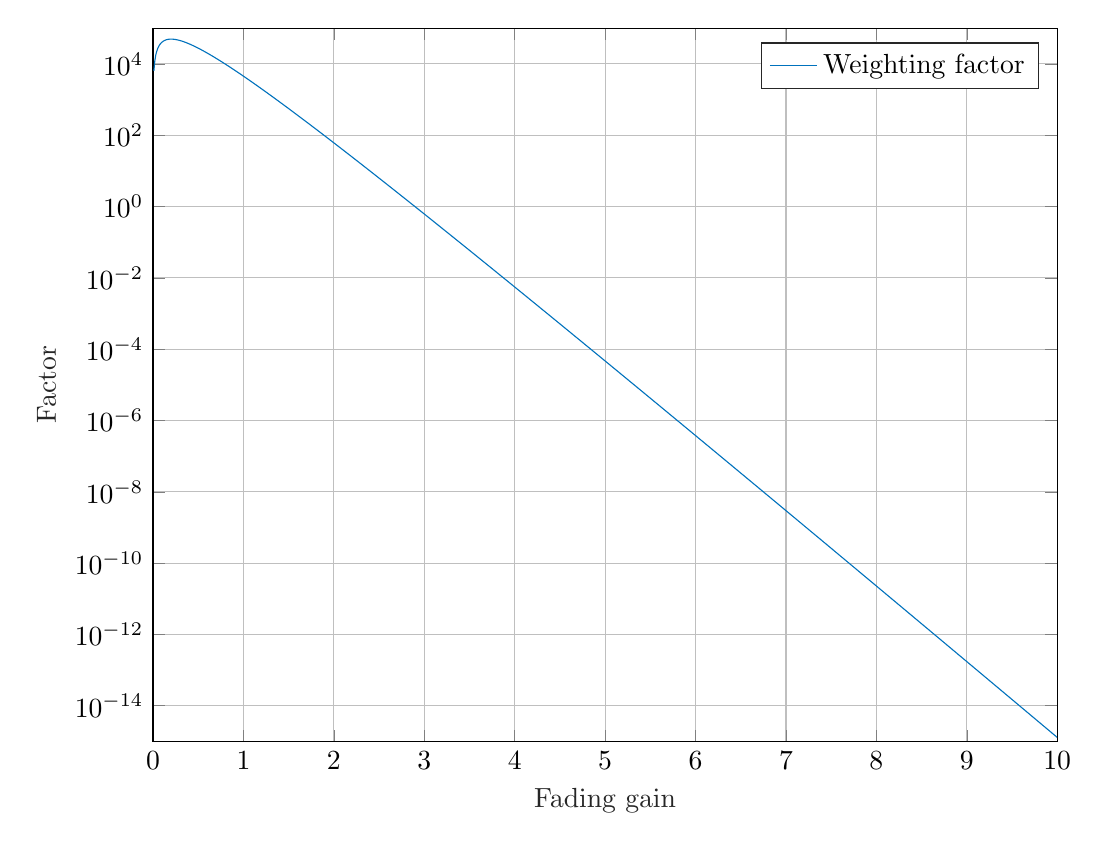
\begin{tikzpicture}

\begin{axis}[%
width=4.521in,
height=3.566in,
at={(0.758in,0.481in)},
scale only axis,
xmin=0,
xmax=10,
xlabel style={font=\color{white!15!black}},
xlabel={Fading gain},
ymode=log,
ymin=1e-15,
ymax=100000,
yminorticks=true,
ylabel style={font=\color{white!15!black}},
ylabel={Factor},
axis background/.style={fill=white},
xmajorgrids,
ymajorgrids,
yminorgrids,
legend style={legend cell align=left, align=left, draw=white!15!black}
]
\addplot [color=mycolor1]
  table[row sep=crcr]{%
0.01	6398.17675811376\\
0.02	12172.2679909488\\
0.03	17367.929213848\\
0.04	22027.8470811437\\
0.05	26191.9203774826\\
0.06	29897.4304166896\\
0.07	33179.2014508706\\
0.08	36069.7516588628\\
0.09	38599.4352513867\\
0.1	40796.5762002547\\
0.11	42687.5940706244\\
0.12	44297.1224084948\\
0.13	45648.1201103094\\
0.14	46761.9761776129\\
0.15	47658.6082370857\\
0.16	48356.555184926\\
0.17	48873.0642943563\\
0.18	49224.1731059721\\
0.19	49424.7864026237\\
0.2	49488.7485535143\\
0.21	49428.9114961109\\
0.22	49257.198609292\\
0.23	48984.6647167993\\
0.24	48621.5524465267\\
0.25	48177.345158376\\
0.26	47660.8166413333\\
0.27	47080.0777690069\\
0.28	46442.620292093\\
0.29	45755.3579360655\\
0.3	45024.6649627736\\
0.31	44256.4123455724\\
0.32	43456.00169904\\
0.33	42628.3970962574\\
0.34	41778.1548989961\\
0.35	40909.4517189583\\
0.36	40026.1106214148\\
0.37	39131.6256761717\\
0.38	38229.1849547417\\
0.39	37321.6920668838\\
0.4	36411.7863242817\\
0.41	35501.8616140467\\
0.42	34594.0840599272\\
0.43	33690.4085445837\\
0.44	32792.5941620131\\
0.45	31902.2186651766\\
0.46	31020.6919700869\\
0.47	30149.2687740223\\
0.48	29289.0603421588\\
0.49	28441.0455137184\\
0.5	27606.0809757275\\
0.51	26784.9108496467\\
0.52	25978.1756334557\\
0.53	25186.4205392634\\
0.54	24410.1032641323\\
0.55	23649.6012295722\\
0.56	22905.2183230459\\
0.57	22177.1911728423\\
0.58	21465.6949857954\\
0.59	20770.8489755675\\
0.6	20092.7214075461\\
0.61	19431.3342848391\\
0.62	18786.6676983772\\
0.63	18158.6638627395\\
0.64	17547.2308580121\\
0.65	16952.2460967518\\
0.66	16373.5595339709\\
0.67	15810.9966369596\\
0.68	15264.3611307393\\
0.69	14733.4375339666\\
0.7	14217.9934991979\\
0.71	13717.7819705655\\
0.72	13232.5431711082\\
0.73	12762.0064312415\\
0.74	12305.8918691337\\
0.75	11863.9119330852\\
0.76	11435.7728153749\\
0.77	11021.1757464412\\
0.78	10619.8181777073\\
0.79	10231.394860835\\
0.8	9855.59883069538\\
0.81	9492.12229888016\\
0.82	9140.65746414373\\
0.83	8800.89724575092\\
0.84	8472.5359453242\\
0.85	8155.26984241965\\
0.86	7848.7977287217\\
0.87	7552.82138542742\\
0.88	7267.04600809057\\
0.89	6991.18058291549\\
0.9	6724.93821822531\\
0.91	6468.03643458227\\
0.92	6220.19741680435\\
0.93	5981.14823090532\\
0.94	5750.62100877988\\
0.95	5528.35310326407\\
0.96	5314.08721602151\\
0.97	5107.57150053694\\
0.98	4908.55964234118\\
0.99	4716.81091844339\\
1	4532.09023780767\\
1.01	4354.16816458205\\
1.02	4182.82092566555\\
1.03	4017.83040408597\\
1.04	3858.98411955435\\
1.05	3706.07519746263\\
1.06	3558.90232749816\\
1.07	3417.26971296146\\
1.08	3280.9870117925\\
1.09	3149.86927023486\\
1.1	3023.73684999614\\
1.11	2902.41534969673\\
1.12	2785.73552133743\\
1.13	2673.53318245848\\
1.14	2565.64912460906\\
1.15	2461.92901869608\\
1.16	2362.22331773427\\
1.17	2266.38715747632\\
1.18	2174.280255361\\
1.19	2085.76680817989\\
1.2	2000.71538882788\\
1.21	1918.99884247034\\
1.22	1840.49418242936\\
1.23	1765.08248606353\\
1.24	1692.64879088942\\
1.25	1623.08199116892\\
1.26	1556.2747351641\\
1.27	1492.12332324035\\
1.28	1430.52760697954\\
1.29	1371.39088944703\\
1.3	1314.61982673991\\
1.31	1260.12433092878\\
1.32	1207.81747449124\\
1.33	1157.61539632253\\
1.34	1109.43720939672\\
1.35	1063.20491014109\\
1.36	1018.84328957614\\
1.37	976.27984626463\\
1.38	935.444701104562\\
1.39	896.27051399324\\
1.4	858.692402382624\\
1.41	822.647861739713\\
1.42	788.076687919831\\
1.43	754.920901455455\\
1.44	723.124673758355\\
1.45	692.634255228519\\
1.46	663.397905259406\\
1.47	635.365824125534\\
1.48	608.490086735321\\
1.49	582.724578229221\\
1.5	558.024931400742\\
1.51	534.348465915734\\
1.52	511.654129303385\\
1.53	489.902439690677\\
1.54	469.055430250606\\
1.55	449.076595333207\\
1.56	429.930838247388\\
1.57	411.584420660667\\
1.58	394.00491358321\\
1.59	377.161149901997\\
1.6	361.023178430494\\
1.61	345.562219438919\\
1.62	330.750621629961\\
1.63	316.561820524756\\
1.64	302.970298223881\\
1.65	289.951544508241\\
1.66	277.482019244853\\
1.67	265.53911606278\\
1.68	254.101127264735\\
1.69	243.147209940237\\
1.7	232.657353246562\\
1.71	222.612346824202\\
1.72	212.993750313979\\
1.73	203.783863943492\\
1.74	194.965700151104\\
1.75	186.522956216206\\
1.76	178.439987865129\\
1.77	170.701783822616\\
1.78	163.293941279413\\
1.79	156.202642247151\\
1.8	149.414630772317\\
1.81	142.917190981768\\
1.82	136.698125932873\\
1.83	130.74573724201\\
1.84	125.048805465823\\
1.85	119.596571210244\\
1.86	114.378716942982\\
1.87	109.385349485775\\
1.88	104.606983163373\\
1.89	100.034523586832\\
1.9	95.6592520493337\\
1.91	91.4728105133461\\
1.92	87.4671871685761\\
1.93	83.6347025407331\\
1.94	79.9679961317374\\
1.95	76.4600135725734\\
1.96	73.1039942705607\\
1.97	69.8934595333762\\
1.98	66.8222011527049\\
1.99	63.884270430936\\
2	61.0739676348415\\
2.01	58.3858318606919\\
2.02	55.8146312957609\\
2.03	53.3553538616624\\
2.04	51.0031982254367\\
2.05	48.7535651647745\\
2.06	46.6020492742125\\
2.07	44.5444309995839\\
2.08	42.5766689884287\\
2.09	40.6948927444965\\
2.1	38.8953955748698\\
2.11	37.1746278186416\\
2.12	35.5291903464568\\
2.13	33.9558283206055\\
2.14	32.4514252057131\\
2.15	31.0129970204279\\
2.16	29.6376868208434\\
2.17	28.3227594067257\\
2.18	27.0655962419334\\
2.19	25.8636905807306\\
2.2	24.714642791991\\
2.21	23.6161558735835\\
2.22	22.5660311495097\\
2.23	21.5621641426386\\
2.24	20.6025406161427\\
2.25	19.6852327769993\\
2.26	18.8083956351638\\
2.27	17.9702635122603\\
2.28	17.1691466938666\\
2.29	16.4034282196908\\
2.3	15.6715608061515\\
2.31	14.9720638960837\\
2.32	14.3035208304876\\
2.33	13.6645761374356\\
2.34	13.0539329334361\\
2.35	12.4703504327337\\
2.36	11.9126415601981\\
2.37	11.3796706636227\\
2.38	10.8703513214135\\
2.39	10.3836442418055\\
2.4	9.91855524989398\\
2.41	9.47413335891116\\
2.42	9.04946892231909\\
2.43	8.64369186342383\\
2.44	8.25596997934446\\
2.45	7.88550731629514\\
2.46	7.53154261325877\\
2.47	7.1933478112453\\
2.48	6.87022662543983\\
2.49	6.56151317765139\\
2.5	6.2665706865775\\
2.51	5.98479021349731\\
2.52	5.71558946110248\\
2.53	5.45841162326593\\
2.54	5.21272428363701\\
2.55	4.97801836103645\\
2.56	4.75380709970591\\
2.57	4.53962510254551\\
2.58	4.33502740554781\\
2.59	4.13958859170963\\
2.6	3.95290194277233\\
2.61	3.77457862720851\\
2.62	3.60424692293704\\
2.63	3.44155147331068\\
2.64	3.2861525749794\\
2.65	3.1377254962901\\
2.66	2.99595982493791\\
2.67	2.86055884363718\\
2.68	2.73123893263055\\
2.69	2.60772899790361\\
2.7	2.48976992401863\\
2.71	2.37711405052626\\
2.72	2.2695246709567\\
2.73	2.16677555343345\\
2.74	2.06865048199205\\
2.75	1.9749428177247\\
2.76	1.88545507890764\\
2.77	1.79999853930383\\
2.78	1.71839284386666\\
2.79	1.64046564110266\\
2.8	1.56605223138279\\
2.81	1.49499523052059\\
2.82	1.42714424796496\\
2.83	1.3623555789821\\
2.84	1.30049191022748\\
2.85	1.24142203813399\\
2.86	1.18502059956651\\
2.87	1.13116781421619\\
2.88	1.07974923823001\\
2.89	1.03065552859247\\
2.9	0.983782217796656\\
2.91	0.939029498361399\\
2.92	0.896302016770202\\
2.93	0.855508676425363\\
2.94	0.816562449228161\\
2.95	0.779380195412306\\
2.96	0.743882491273876\\
2.97	0.709993464455979\\
2.98	0.677640636461049\\
2.99	0.646754772077527\\
3	0.617269735421134\\
3.01	0.589122352303642\\
3.02	0.5622522786544\\
3.03	0.536601874731583\\
3.04	0.512116084871373\\
3.05	0.48874232253413\\
3.06	0.466430360416867\\
3.07	0.445132225411314\\
3.08	0.424802098196272\\
3.09	0.405396217262098\\
3.1	0.386872787173811\\
3.11	0.369191890887681\\
3.12	0.352315405944111\\
3.13	0.336206924367283\\
3.14	0.32083167610933\\
3.15	0.306156455883851\\
3.16	0.292149553240233\\
3.17	0.278780685736711\\
3.18	0.26602093507624\\
3.19	0.253842686075128\\
3.2	0.242219568340022\\
3.21	0.23112640053425\\
3.22	0.220539137119661\\
3.23	0.210434817465084\\
3.24	0.200791517217216\\
3.25	0.19158830183434\\
3.26	0.182805182187548\\
3.27	0.174423072138341\\
3.28	0.166423748005427\\
3.29	0.158789809837352\\
3.3	0.151504644411226\\
3.31	0.144552389881302\\
3.32	0.137917902004477\\
3.33	0.131586721873004\\
3.34	0.12554504508772\\
3.35	0.11977969230803\\
3.36	0.1142780811177\\
3.37	0.109028199148132\\
3.38	0.104018578403409\\
3.39	0.099238270733809\\
3.4	0.0946768244068227\\
3.41	0.0903242617269806\\
3.42	0.0861710576579023\\
3.43	0.0822081194020428\\
3.44	0.0784267668955784\\
3.45	0.0748187141777289\\
3.46	0.0713760515956258\\
3.47	0.0680912288075342\\
3.48	0.0649570385488869\\
3.49	0.0619666011271517\\
3.5	0.0591133496130546\\
3.51	0.0563910156971147\\
3.52	0.0537936161818209\\
3.53	0.0513154400810891\\
3.54	0.0489510362998943\\
3.55	0.0466952018681724\\
3.56	0.0445429707042316\\
3.57	0.0424896028840118\\
3.58	0.0405305743935766\\
3.59	0.0386615673432279\\
3.6	0.0368784606225903\\
3.61	0.0351773209769281\\
3.62	0.0335543944858348\\
3.63	0.0320060984262754\\
3.64	0.0305290135027555\\
3.65	0.0291198764281655\\
3.66	0.0277755728395733\\
3.67	0.0264931305339425\\
3.68	0.0252697130094196\\
3.69	0.0241026132984746\\
3.7	0.0229892480797896\\
3.71	0.0219271520563739\\
3.72	0.0209139725879434\\
3.73	0.0199474645661349\\
3.74	0.0190254855216363\\
3.75	0.0181459909528003\\
3.76	0.0173070298657768\\
3.77	0.0165067405166433\\
3.78	0.0157433463464378\\
3.79	0.0150151521004058\\
3.8	0.0143205401231628\\
3.81	0.0136579668218426\\
3.82	0.0130259592896594\\
3.83	0.012423112082648\\
3.84	0.0118480841426734\\
3.85	0.0112995958601079\\
3.86	0.0107764262698728\\
3.87	0.010277410374821\\
3.88	0.00980143659071083\\
3.89	0.00934744430727514\\
3.9	0.00891442156014167\\
3.91	0.00850140280859084\\
3.92	0.00810746681436659\\
3.93	0.00773173461696812\\
3.94	0.00737336760105799\\
3.95	0.00703156565181651\\
3.96	0.00670556539426152\\
3.97	0.00639463851273058\\
3.98	0.00609809014689475\\
3.99	0.00581525736083588\\
4	0.00554550768187615\\
4.01	0.00528823770599733\\
4.02	0.00504287176683024\\
4.03	0.0048088606653306\\
4.04	0.00458568045738802\\
4.05	0.00437283129673831\\
4.06	0.00416983633066926\\
4.07	0.00397624064612183\\
4.08	0.00379161026389834\\
4.09	0.00361553117879152\\
4.1	0.00344760844354807\\
4.11	0.00328746529467383\\
4.12	0.00313474231817832\\
4.13	0.00298909665344209\\
4.14	0.00285020123347294\\
4.15	0.0027177440598949\\
4.16	0.00259142751108956\\
4.17	0.00247096768198022\\
4.18	0.00235609375401819\\
4.19	0.0022465473939956\\
4.2	0.00214208218037156\\
4.21	0.00204246305585777\\
4.22	0.00194746580506686\\
4.23	0.00185687655608095\\
4.24	0.00177049130484949\\
4.25	0.00168811546137521\\
4.26	0.00160956341669426\\
4.27	0.00153465812970165\\
4.28	0.0014632307329161\\
4.29	0.00139512015631995\\
4.3	0.00133017276844848\\
4.31	0.00126824203394107\\
4.32	0.00120918818680208\\
4.33	0.00115287791865371\\
4.34	0.00109918408129551\\
4.35	0.00104798540291686\\
4.36	0.000999166217337849\\
4.37	0.00095261620568301\\
4.38	0.000908230149919071\\
4.39	0.000865907697714003\\
4.4	0.000825553138099271\\
4.41	0.000787075187440859\\
4.42	0.000750386785247089\\
4.43	0.000715404899362906\\
4.44	0.000682050340120652\\
4.45	0.000650247583037163\\
4.46	0.000619924599665524\\
4.47	0.000591012696227873\\
4.48	0.00056344635967258\\
4.49	0.000537163110815443\\
4.5	0.000512103364240077\\
4.51	0.000488210294647526\\
4.52	0.000465429709359261\\
4.53	0.000443709926691244\\
4.54	0.000423001659929674\\
4.55	0.00040325790665127\\
4.56	0.000384433843142809\\
4.57	0.000366486723685742\\
4.58	0.000349375784482501\\
4.59	0.000333062152011286\\
4.6	0.000317508755605896\\
4.61	0.000302680244066474\\
4.62	0.000288542906115928\\
4.63	0.000275064594525233\\
4.64	0.00026221465373899\\
4.65	0.000249963850840266\\
4.66	0.000238284309701158\\
4.67	0.000227149448172532\\
4.68	0.000216533918173149\\
4.69	0.00020641354854473\\
4.7	0.000196765290545706\\
4.71	0.000187567165862162\\
4.72	0.000178798217020117\\
4.73	0.000170438460088557\\
4.74	0.000162468839567737\\
4.75	0.00015487118536208\\
4.76	0.00014762817174166\\
4.77	0.00014072327820063\\
4.78	0.000134140752125185\\
4.79	0.000127865573187652\\
4.8	0.000121883419387134\\
4.81	0.000116180634660802\\
4.82	0.000110744197993397\\
4.83	0.000105561693955845\\
4.84	0.000100621284607069\\
4.85	9.59116826961009e-05\\
4.86	9.14221261044923e-05\\
4.87	8.71423534717919e-05\\
4.88	8.30625809494742e-05\\
4.89	7.91734800312315e-05\\
4.9	7.54661564099287e-05\\
4.91	7.1932129813814e-05\\
4.92	6.85633147767521e-05\\
4.93	6.53520022993434e-05\\
4.94	6.22908423597642e-05\\
4.95	5.93728272350687e-05\\
4.96	5.65912755954953e-05\\
4.97	5.3939817336054e-05\\
4.98	5.1412379111307e-05\\
4.99	4.90031705408359e-05\\
5	4.67066710543785e-05\\
5.01	4.45176173470555e-05\\
5.02	4.24309914164665e-05\\
5.03	4.04420091547375e-05\\
5.04	3.85461094698458e-05\\
5.05	3.67389439117266e-05\\
5.06	3.50163667798047e-05\\
5.07	3.33744256896643e-05\\
5.08	3.1809352577604e-05\\
5.09	3.03175551228002e-05\\
5.1	2.88956085677451e-05\\
5.11	2.75402479185106e-05\\
5.12	2.62483605072476e-05\\
5.13	2.50169789001374e-05\\
5.14	2.38432741347935e-05\\
5.15	2.27245492718442e-05\\
5.16	2.1658233246139e-05\\
5.17	2.06418750036876e-05\\
5.18	1.96731379110898e-05\\
5.19	1.87497944248205e-05\\
5.2	1.78697210083217e-05\\
5.21	1.70308932854087e-05\\
5.22	1.6231381419032e-05\\
5.23	1.54693457049395e-05\\
5.24	1.47430323702707e-05\\
5.25	1.4050769567573e-05\\
5.26	1.33909635551728e-05\\
5.27	1.27620950552531e-05\\
5.28	1.21627157813875e-05\\
5.29	1.15914451276652e-05\\
5.3	1.10469670119053e-05\\
5.31	1.05280268658041e-05\\
5.32	1.00334287651928e-05\\
5.33	9.56203269389924e-06\\
5.34	9.11275193500476e-06\\
5.35	8.68455058358148e-06\\
5.36	8.27644117526315e-06\\
5.37	7.88748242526867e-06\\
5.38	7.516777072744e-06\\
5.39	7.16346982552876e-06\\
5.4	6.82674540067829e-06\\
5.41	6.50582665629031e-06\\
5.42	6.19997281039024e-06\\
5.43	5.90847774282794e-06\\
5.44	5.63066837632431e-06\\
5.45	5.36590313298735e-06\\
5.46	5.11357046278625e-06\\
5.47	4.87308744063668e-06\\
5.48	4.6438984289045e-06\\
5.49	4.42547380228406e-06\\
5.5	4.21730873214811e-06\\
5.51	4.01892202760167e-06\\
5.52	3.82985503060017e-06\\
5.53	3.64967056261496e-06\\
5.54	3.47795192044658e-06\\
5.55	3.31430191889674e-06\\
5.56	3.15834197811743e-06\\
5.57	3.00971125355601e-06\\
5.58	2.86806580651246e-06\\
5.59	2.73307781341666e-06\\
5.6	2.60443481202204e-06\\
5.61	2.48183898279539e-06\\
5.62	2.36500646386282e-06\\
5.63	2.25366669794782e-06\\
5.64	2.14756180981067e-06\\
5.65	2.04644601276709e-06\\
5.66	1.95008504293073e-06\\
5.67	1.85825561988674e-06\\
5.68	1.77074493256417e-06\\
5.69	1.68735014913201e-06\\
5.7	1.60787794979846e-06\\
5.71	1.53214408144515e-06\\
5.72	1.4599729330779e-06\\
5.73	1.39119713112271e-06\\
5.74	1.32565715364121e-06\\
5.75	1.26320096258265e-06\\
5.76	1.20368365323088e-06\\
5.77	1.14696712004363e-06\\
5.78	1.09291973811917e-06\\
5.79	1.04141605956072e-06\\
5.8	9.92336524043192e-07\\
5.81	9.45567182919192e-07\\
5.82	9.00999436231943e-07\\
5.83	8.58529782032626e-07\\
5.84	8.18059577427269e-07\\
5.85	7.79494810805499e-07\\
5.86	7.42745884728735e-07\\
5.87	7.07727408979902e-07\\
5.88	6.74358003299887e-07\\
5.89	6.42560109358147e-07\\
5.9	6.12259811525977e-07\\
5.91	5.83386666041013e-07\\
5.92	5.55873538170818e-07\\
5.93	5.29656447001649e-07\\
5.94	5.04674417495944e-07\\
5.95	4.8086933947873e-07\\
5.96	4.58185833228951e-07\\
5.97	4.36571121366918e-07\\
5.98	4.15974906743429e-07\\
5.99	3.96349256049875e-07\\
6	3.77648488881746e-07\\
6.01	3.59829072000452e-07\\
6.02	3.42849518550292e-07\\
6.03	3.26670291998716e-07\\
6.04	3.1125371457892e-07\\
6.05	2.9656388002406e-07\\
6.06	2.8256657039228e-07\\
6.07	2.69229176791081e-07\\
6.08	2.56520623818535e-07\\
6.09	2.4441129754735e-07\\
6.1	2.32872976885941e-07\\
6.11	2.21878768158398e-07\\
6.12	2.1140304275266e-07\\
6.13	2.01421377693181e-07\\
6.14	1.91910499001189e-07\\
6.15	1.82848227711947e-07\\
6.16	1.74213428424594e-07\\
6.17	1.65985960265916e-07\\
6.18	1.58146630154989e-07\\
6.19	1.50677148260884e-07\\
6.2	1.43560085550691e-07\\
6.21	1.36778833329915e-07\\
6.22	1.3031756468188e-07\\
6.23	1.24161197717146e-07\\
6.24	1.18295360548114e-07\\
6.25	1.1270635790794e-07\\
6.26	1.07381139336694e-07\\
6.27	1.02307268861292e-07\\
6.28	9.74728960991582e-08\\
6.29	9.28667287188787e-08\\
6.3	8.84780061941964e-08\\
6.31	8.42964747907161e-08\\
6.32	8.03123637274966e-08\\
6.33	7.6516362458433e-08\\
6.34	7.28995990208935e-08\\
6.35	6.94536194015625e-08\\
6.36	6.61703678717576e-08\\
6.37	6.30421682467432e-08\\
6.38	6.00617060256827e-08\\
6.39	5.72220113709108e-08\\
6.4	5.45164428871357e-08\\
6.41	5.19386721630333e-08\\
6.42	4.94826690394462e-08\\
6.43	4.71426875700882e-08\\
6.44	4.49132526422432e-08\\
6.45	4.27891472264781e-08\\
6.46	4.0765400225834e-08\\
6.47	3.88372748963558e-08\\
6.48	3.70002578121267e-08\\
6.49	3.52500483492435e-08\\
6.5	3.35825486643569e-08\\
6.51	3.19938541445546e-08\\
6.52	3.04802443064453e-08\\
6.53	2.90381741233443e-08\\
6.54	2.76642657604515e-08\\
6.55	2.63553006988527e-08\\
6.56	2.51082122300783e-08\\
6.57	2.39200783038071e-08\\
6.58	2.2788114712122e-08\\
6.59	2.17096685945012e-08\\
6.6	2.06822122484736e-08\\
6.61	1.97033372315694e-08\\
6.62	1.8770748740878e-08\\
6.63	1.78822602571608e-08\\
6.64	1.70357884410843e-08\\
6.65	1.62293482697205e-08\\
6.66	1.54610484020183e-08\\
6.67	1.47290867624789e-08\\
6.68	1.40317463327765e-08\\
6.69	1.33673911415449e-08\\
6.7	1.27344624430104e-08\\
6.71	1.21314750755893e-08\\
6.72	1.15570139919856e-08\\
6.73	1.10097309527225e-08\\
6.74	1.04883413754182e-08\\
6.75	9.99162133248014e-09\\
6.76	9.51840469023516e-09\\
6.77	9.0675803828402e-09\\
6.78	8.63808981463234e-09\\
6.79	8.22892438487377e-09\\
6.8	7.83912312913212e-09\\
6.81	7.46777047180681e-09\\
6.82	7.11399408457052e-09\\
6.83	6.7769628457402e-09\\
6.84	6.45588489582645e-09\\
6.85	6.15000578473451e-09\\
6.86	5.85860670630114e-09\\
6.87	5.58100281605637e-09\\
6.88	5.31654162829064e-09\\
6.89	5.06460148869411e-09\\
6.9	4.82459011900871e-09\\
6.91	4.59594323030194e-09\\
6.92	4.37812320163048e-09\\
6.93	4.17061782101412e-09\\
6.94	3.97293908578471e-09\\
6.95	3.78462205951358e-09\\
6.96	3.60522378285205e-09\\
6.97	3.43432223574508e-09\\
6.98	3.2715153485979e-09\\
6.99	3.11642006008902e-09\\
7	2.96867141943158e-09\\
7.01	2.82792173098882e-09\\
7.02	2.69383973924749e-09\\
7.03	2.56610985224738e-09\\
7.04	2.44443140165442e-09\\
7.05	2.32851793775026e-09\\
7.06	2.21809655769253e-09\\
7.07	2.11290726547739e-09\\
7.08	2.01270236210992e-09\\
7.09	1.91724586455812e-09\\
7.1	1.82631295213356e-09\\
7.11	1.73968943900552e-09\\
7.12	1.65717127161623e-09\\
7.13	1.57856404982306e-09\\
7.14	1.50368257064881e-09\\
7.15	1.43235039357376e-09\\
7.16	1.36439942635354e-09\\
7.17	1.29966953039469e-09\\
7.18	1.23800814476542e-09\\
7.19	1.17926992796248e-09\\
7.2	1.12331641659647e-09\\
7.21	1.0700157001975e-09\\
7.22	1.01924211138064e-09\\
7.23	9.70875930646347e-10\\
7.24	9.24803105125468e-10\\
7.25	8.80914980610642e-10\\
7.26	8.39108046247271e-10\\
7.27	7.99283691286492e-10\\
7.28	7.61347973330927e-10\\
7.29	7.25211397530809e-10\\
7.3	6.90788706213513e-10\\
7.31	6.57998678454119e-10\\
7.32	6.26763939117644e-10\\
7.33	5.97010776925859e-10\\
7.34	5.68668971122562e-10\\
7.35	5.41671626331419e-10\\
7.36	5.15955015219496e-10\\
7.37	4.91458428597938e-10\\
7.38	4.68124032608572e-10\\
7.39	4.4589673266184e-10\\
7.4	4.24724043807221e-10\\
7.41	4.04555967232308e-10\\
7.42	3.8534487260112e-10\\
7.43	3.67045385955805e-10\\
7.44	3.49614282918971e-10\\
7.45	3.33010386946225e-10\\
7.46	3.17194472390339e-10\\
7.47	3.02129172149762e-10\\
7.48	2.87778889684837e-10\\
7.49	2.74109715195392e-10\\
7.5	2.61089345763052e-10\\
7.51	2.48687009270941e-10\\
7.52	2.36873391922263e-10\\
7.53	2.2562056918769e-10\\
7.54	2.149019400195e-10\\
7.55	2.04692164178078e-10\\
7.56	1.94967102523675e-10\\
7.57	1.85703760133249e-10\\
7.58	1.76880232108864e-10\\
7.59	1.68475651950397e-10\\
7.6	1.60470142371332e-10\\
7.61	1.52844768442137e-10\\
7.62	1.45581492951179e-10\\
7.63	1.38663133878322e-10\\
7.64	1.32073323881318e-10\\
7.65	1.25796471699809e-10\\
7.66	1.19817725386262e-10\\
7.67	1.14122937277428e-10\\
7.68	1.0869863062403e-10\\
7.69	1.03531967800237e-10\\
7.7	9.86107200181989e-11\\
7.71	9.3923238476477e-11\\
7.72	8.94584268745107e-11\\
7.73	8.52057152285289e-11\\
7.74	8.11550349273197e-11\\
7.75	7.72967949692099e-11\\
7.76	7.36218593243685e-11\\
7.77	7.01215253691883e-11\\
7.78	6.67875033420219e-11\\
7.79	6.36118967719429e-11\\
7.8	6.0587183834485e-11\\
7.81	5.77061995904975e-11\\
7.82	5.49621190663187e-11\\
7.83	5.23484411354551e-11\\
7.84	4.98589731638241e-11\\
7.85	4.74878163824291e-11\\
7.86	4.52293519530283e-11\\
7.87	4.3078227693996e-11\\
7.88	4.10293454351232e-11\\
7.89	3.90778489715862e-11\\
7.9	3.72191125887128e-11\\
7.91	3.5448730130528e-11\\
7.92	3.37625045863261e-11\\
7.93	3.21564381707468e-11\\
7.94	3.06267228739859e-11\\
7.95	2.91697314598776e-11\\
7.96	2.77820088906391e-11\\
7.97	2.64602641580748e-11\\
7.98	2.52013625019867e-11\\
7.99	2.40023179974556e-11\\
8	2.28602864935198e-11\\
8.01	2.17725588866087e-11\\
8.02	2.07365547128747e-11\\
8.03	1.97498160443158e-11\\
8.04	1.88100016743e-11\\
8.05	1.79148815787797e-11\\
8.06	1.70623316401365e-11\\
8.07	1.62503286212118e-11\\
8.08	1.54769453776713e-11\\
8.09	1.47403462974093e-11\\
8.1	1.4038782956236e-11\\
8.11	1.33705899795979e-11\\
8.12	1.27341811005681e-11\\
8.13	1.21280454048055e-11\\
8.14	1.15507437536232e-11\\
8.15	1.10009053767212e-11\\
8.16	1.04772246265473e-11\\
8.17	9.97845788662025e-12\\
8.18	9.50342062652094e-12\\
8.19	9.0509845965974e-12\\
8.2	8.62007515576149e-12\\
8.21	8.20966872606735e-12\\
8.22	7.818790368062e-12\\
8.23	7.44651147118136e-12\\
8.24	7.09194755373794e-12\\
8.25	6.75425616730386e-12\\
8.26	6.43263490053905e-12\\
8.27	6.12631947774923e-12\\
8.28	5.8345819476821e-12\\
8.29	5.55672895828176e-12\\
8.3	5.2921001133257e-12\\
8.31	5.04006640706065e-12\\
8.32	4.80002873313795e-12\\
8.33	4.57141646432486e-12\\
8.34	4.35368609963471e-12\\
8.35	4.14631997567776e-12\\
8.36	3.94882503918704e-12\\
8.37	3.7607316778166e-12\\
8.38	3.58159260644839e-12\\
8.39	3.41098180637425e-12\\
8.4	3.24849351484414e-12\\
8.41	3.09374126259166e-12\\
8.42	2.94635695706022e-12\\
8.43	2.80599000916139e-12\\
8.44	2.67230650150003e-12\\
8.45	2.5449883960985e-12\\
8.46	2.42373277974551e-12\\
8.47	2.30825114518446e-12\\
8.48	2.19826870643981e-12\\
8.49	2.09352374666209e-12\\
8.5	1.99376699694766e-12\\
8.51	1.89876104466339e-12\\
8.52	1.80827976987563e-12\\
8.53	1.72210780854967e-12\\
8.54	1.64004004124886e-12\\
8.55	1.5618811061229e-12\\
8.56	1.48744493503246e-12\\
8.57	1.41655431171145e-12\\
8.58	1.34904045092115e-12\\
8.59	1.28474259759912e-12\\
8.6	1.22350764505396e-12\\
8.61	1.16518977130141e-12\\
8.62	1.10965009268044e-12\\
8.63	1.05675633392887e-12\\
8.64	1.00638251393696e-12\\
8.65	9.58408646434328e-13\\
8.66	9.12720454901213e-13\\
8.67	8.69209101028443e-13\\
8.68	8.27770926082714e-13\\
8.69	7.88307204564236e-13\\
8.7	7.50723909572895e-13\\
8.71	7.1493148932684e-13\\
8.72	6.8084465430383e-13\\
8.73	6.48382174500537e-13\\
8.74	6.17466686329469e-13\\
8.75	5.88024508695482e-13\\
8.76	5.5998546781586e-13\\
8.77	5.33282730368605e-13\\
8.78	5.07852644573231e-13\\
8.79	4.83634588827228e-13\\
8.8	4.60570827539145e-13\\
8.81	4.3860637381645e-13\\
8.82	4.17688858682328e-13\\
8.83	3.97768406511308e-13\\
8.84	3.78797516388133e-13\\
8.85	3.60730949108398e-13\\
8.86	3.43525619552882e-13\\
8.87	3.27140494180173e-13\\
8.88	3.11536493394337e-13\\
8.89	2.96676398555936e-13\\
8.9	2.82524763415708e-13\\
8.91	2.69047829760687e-13\\
8.92	2.5621344707256e-13\\
8.93	2.43990996007512e-13\\
8.94	2.32351315515936e-13\\
8.95	2.21266633428955e-13\\
8.96	2.10710500346972e-13\\
8.97	2.00657726673251e-13\\
8.98	1.91084322643016e-13\\
8.99	1.81967441205661e-13\\
9	1.73285323624401e-13\\
9.01	1.65017247664177e-13\\
9.02	1.57143478244744e-13\\
9.03	1.49645220441723e-13\\
9.04	1.42504574723961e-13\\
9.05	1.35704494320873e-13\\
9.06	1.29228744618469e-13\\
9.07	1.23061864487577e-13\\
9.08	1.17189129452402e-13\\
9.09	1.11596516611865e-13\\
9.1	1.06270671230386e-13\\
9.11	1.01198874918681e-13\\
9.12	9.63690153289823e-14\\
9.13	9.17695572926135e-14\\
9.14	8.73895153313321e-14\\
9.15	8.3218427477087e-14\\
9.16	7.92463303379516e-14\\
9.17	7.54637353509465e-14\\
9.18	7.18616061652929e-14\\
9.19	6.84313371023175e-14\\
9.2	6.51647326407832e-14\\
9.21	6.20539878788603e-14\\
9.22	5.90916699262759e-14\\
9.23	5.62707001823722e-14\\
9.24	5.35843374579358e-14\\
9.25	5.10261619006353e-14\\
9.26	4.85900596858371e-14\\
9.27	4.62702084363725e-14\\
9.28	4.40610633365712e-14\\
9.29	4.19573439075195e-14\\
9.3	3.99540214120746e-14\\
9.31	3.80463068596671e-14\\
9.32	3.62296395823424e-14\\
9.33	3.44996763548547e-14\\
9.34	3.28522810329188e-14\\
9.35	3.12835146849548e-14\\
9.36	2.97896261938407e-14\\
9.37	2.83670433062924e-14\\
9.38	2.70123641085712e-14\\
9.39	2.57223489082201e-14\\
9.4	2.44939125024988e-14\\
9.41	2.33241168151117e-14\\
9.42	2.22101638836925e-14\\
9.43	2.1149389181348e-14\\
9.44	2.01392552563546e-14\\
9.45	1.91773456748619e-14\\
9.46	1.82613592521729e-14\\
9.47	1.73891045588657e-14\\
9.48	1.65584946886618e-14\\
9.49	1.57675422755864e-14\\
9.5	1.50143547485425e-14\\
9.51	1.42971298119969e-14\\
9.52	1.36141511420085e-14\\
9.53	1.29637842873448e-14\\
9.54	1.23444727659185e-14\\
9.55	1.17547343472424e-14\\
9.56	1.11931575120436e-14\\
9.57	1.06583980805966e-14\\
9.58	1.01491760017437e-14\\
9.59	9.6642722949436e-15\\
9.6	9.20252613806452e-15\\
9.61	8.76283209397459e-15\\
9.62	8.34413746932098e-15\\
9.63	7.94543979919934e-15\\
9.64	7.56578445171752e-15\\
9.65	7.20426234673972e-15\\
9.66	6.86000778337407e-15\\
9.67	6.53219637102103e-15\\
9.68	6.22004305904918e-15\\
9.69	5.92280026039951e-15\\
9.7	5.63975606464244e-15\\
9.71	5.37023253622584e-15\\
9.72	5.11358409385459e-15\\
9.73	4.86919596713528e-15\\
9.74	4.63648272680546e-15\\
9.75	4.41488688503954e-15\\
9.76	4.20387756249283e-15\\
9.77	4.00294921890305e-15\\
9.78	3.81162044422014e-15\\
9.79	3.62943280738005e-15\\
9.8	3.45594975997501e-15\\
9.81	3.29075559220411e-15\\
9.82	3.13345443861184e-15\\
9.83	2.98366933124253e-15\\
9.84	2.84104129794969e-15\\
9.85	2.7052285037083e-15\\
9.86	2.57590543288043e-15\\
9.87	2.45276211048152e-15\\
9.88	2.33550336058864e-15\\
9.89	2.22384810011992e-15\\
9.9	2.11752866629884e-15\\
9.91	2.01629017619772e-15\\
9.92	1.91988991683103e-15\\
9.93	1.82809676434179e-15\\
9.94	1.74069063089427e-15\\
9.95	1.65746193795176e-15\\
9.96	1.57821111468161e-15\\
9.97	1.5027481202893e-15\\
9.98	1.43089198914047e-15\\
9.99	1.3624703975846e-15\\
10	1.2973192514451e-15\\
};
\addlegendentry{Weighting factor}

\end{axis}
\end{tikzpicture}%
\caption{The weighting factor between the two distribution on \autoref{IMD}}
\label{IMW}
\end{figure}
\end{minipage}
\vspace{1em}

This weighting factor is used to go from the actual distribution to the desired distribution. However this can not be used as the measurements are taken physically with no a priori knowledge of the behaviour of the environment. Another way to look at this is to see the change in distribution as force fully introducing more spots with deep fades, that might be possible but without full knowledge of the changes it will only skew the results.

Most of the other rare event simulations tools (like Stochastic process rare event sampling and Transition path sampling) handle this problem with rare events, by using information about the distribution, to limit the number of samples and by not knowing the distribution, these methods can therefore not be used. 


As no useful statistical method has been found the required number of samples can not be reduced from \autoref{tab:numSample}. Therefore a compromise between the necessary number of samples, the more samples needed the longer it will take, and the confidence level and interval needs to be found. It is chosen to go for a 90\% confidence level and a 1 dB margin, as this is found to be a reasonable compromise. This means that $4.04E+6$ samples should be obtained during the measurement campaign. 

%Reduction of number of samples
%- Important sampling
%- Not useful

\section{Bootstrap Percentile Method}
Another statistically aspect, for which there are different method and techniques, is how to determine the confidence interval at a certain confidence level from the measurements. From the previous section the number of samples needed to attain a confidence level of 90\% and a margin of 1 dB is found. However this is estimated based on theory and has no particular onset in the actual measurements, it is therefore necessary to find a method to evaluate the confidence based on the measurements. The method chosen is the \textit{Bootstrap Percentile Method} \citep{Bootstrap}.

The Bootstrap method works on a surrogate population, a subset from the total sample space, which is considered an estimate of the true sample population \citep{Bootstrap}. This surrogate population will consists of the samples from the measurements campaign. For the sake of further explanations lets call the surrogate population $\mathbf{X}$ consisting of $(X_1, X_2,..X_n)$ and the value that wish to find the confidence around $\hat{\gamma}$. A new subset is now found from the surrogate population, this is done by copying randomly a value from $\mathbf{X}$ and putting it into the new subset $\mathbf{B}$ until $\mathbf{B}$ has the same size as $\mathbf{X}$. The value of $\hat{\gamma_B}$ is then found and the process is repeated a couple thousand times. All the new values of $\hat{\gamma_B}$ can then be sorted and the the desired percentile can be picked so that the lowest and highest values is left out. This will produce a the confidence interval given a confidence level \citep{Bootstrap}. For the measurements the 90 \% confidence level is picked leaving out the top and bottom 5 \% of the sorted values.

\begin{figure}[H]
\centering
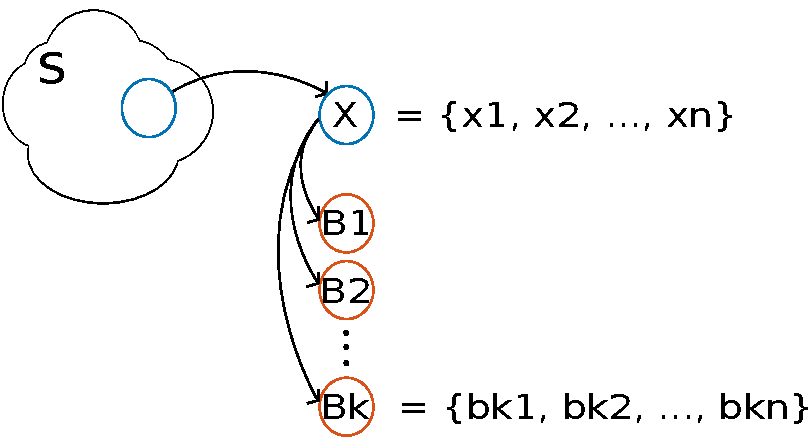
\includegraphics[width=0.5\textwidth]{figures/Bootstrap.pdf}
\caption{Showcase of the bootstrap method, where the surrogate population $X$ is made of samples from the normal sample population $B$. From $X$ there are drawn new subsets $B$, at the same size as $X$.}
\label{BSEX}
\end{figure}

This method is only valid if the assumption of a symmetric distribution around $\hat{\gamma}$ holds \citep{Bootstrap}, which means that a high number of samples is still needed to obtain a sufficient resolution of the CDF. 

An example have been simulated in matlab, where there have been taken $4.04 \cdot 10^6$ sample from $raylrnd$. These values are converted to dB, which give a CDF, which is the yellow line in \autoref{BS90}. By using the booth strap method 10.000 times and make a CDF for each trial. By taking the 500th highest and lowest value in each point in the CDF (which gives a 90\% confidence level), a interval is created, which is shown in \autoref{BS90}. It is seen that at low procentence level, that the interval becomes wider, as there is a less sample population for that part. At the $10^{-5}$ point, there is a interval on 1.63 dB, which lower than the wanted confidence interval for this number of samples. 

\begin{figure}[H]
\center
% This file was created by matlab2tikz.
%
%The latest updates can be retrieved from
%  http://www.mathworks.com/matlabcentral/fileexchange/22022-matlab2tikz-matlab2tikz
%where you can also make suggestions and rate matlab2tikz.
%
\definecolor{mycolor1}{rgb}{0.00000,0.44700,0.74100}%
\definecolor{mycolor2}{rgb}{0.85000,0.32500,0.09800}%
\definecolor{mycolor3}{rgb}{0.92900,0.69400,0.12500}%
%
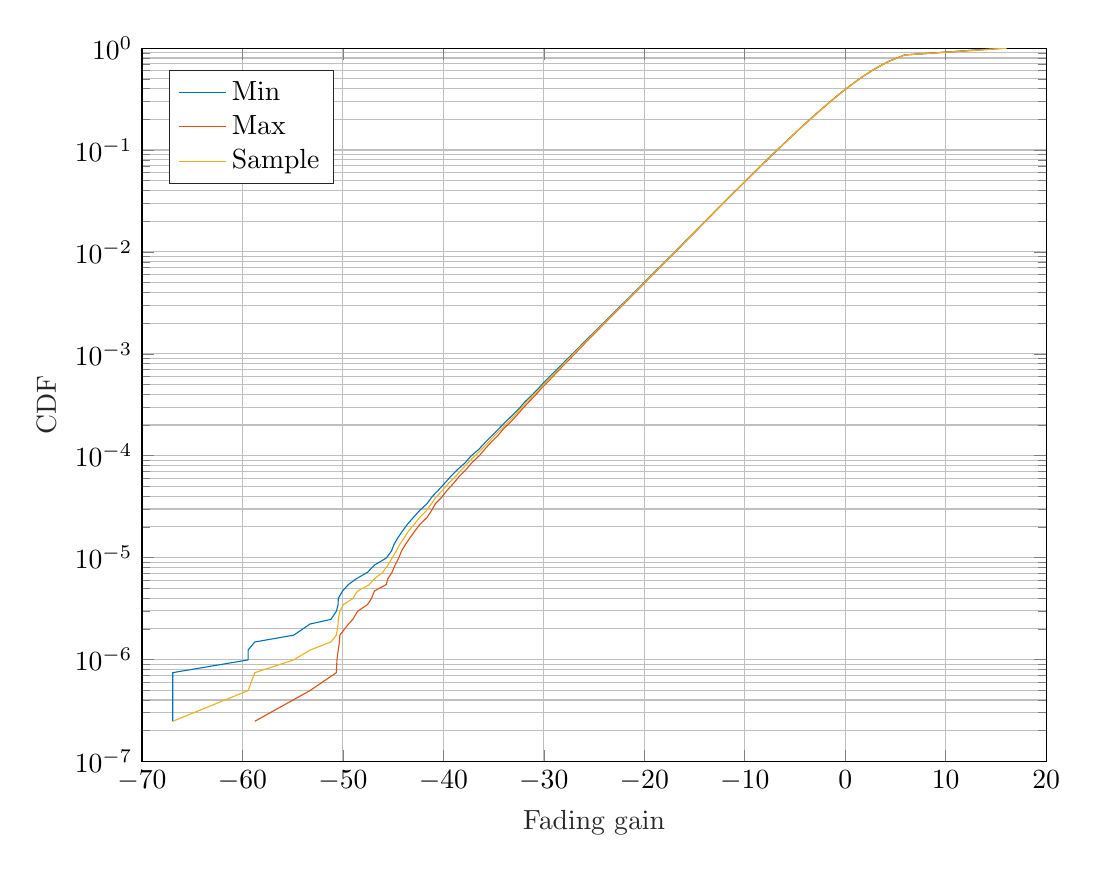
\begin{tikzpicture}

\begin{axis}[%
width=4.521in,
height=3.566in,
at={(0.758in,0.481in)},
scale only axis,
xmin=-70,
xmax=20,
xlabel style={font=\color{white!15!black}},
xlabel={Fading gain},
ymode=log,
ymin=1e-07,
ymax=1,
yminorticks=true,
ylabel style={font=\color{white!15!black}},
ylabel={CDF},
axis background/.style={fill=white},
xmajorgrids,
ymajorgrids,
yminorgrids,
legend style={at={(0.03,0.97)}, anchor=north west, legend cell align=left, align=left, draw=white!15!black}
]
\addplot [color=mycolor1]
  table[row sep=crcr]{%
-66.9341548867478	2.47524752475248e-07\\
-66.9341548867478	2.47524752475248e-07\\
-66.9341548867478	2.47524752475248e-07\\
-66.9341548867478	4.95049504950495e-07\\
-66.9341548867478	4.95049504950495e-07\\
-66.9341548867478	4.95049504950495e-07\\
-66.9341548867478	7.42574257425743e-07\\
-66.9341548867478	7.42574257425743e-07\\
-66.9341548867478	7.42574257425743e-07\\
-59.4401305500329	9.9009900990099e-07\\
-59.4401305500329	1.23762376237624e-06\\
-59.4401305500329	1.23762376237624e-06\\
-58.7667416700321	1.48514851485149e-06\\
-54.8930241094094	1.73267326732673e-06\\
-53.273131300811	2.22772277227723e-06\\
-51.1950865851036	2.47524752475248e-06\\
-50.6510586185259	2.97029702970297e-06\\
-50.4744372709179	3.46534653465347e-06\\
-50.4637174371534	3.96039603960396e-06\\
-50.0349816474052	4.7029702970297e-06\\
-49.447561740496	5.44554455445545e-06\\
-48.6769735680418	6.18811881188119e-06\\
-47.5399711931716	7.17821782178218e-06\\
-46.8753928436756	8.41584158415842e-06\\
-45.6763991666034	9.9009900990099e-06\\
-45.1564337798158	1.16336633663366e-05\\
-44.9298596668173	1.33663366336634e-05\\
-44.5379088207656	1.55940594059406e-05\\
-44.0575718584017	1.83168316831683e-05\\
-43.5660734665178	2.12871287128713e-05\\
-42.9948512600283	2.47524752475248e-05\\
-42.3622899660794	2.8960396039604e-05\\
-41.6199358073098	3.39108910891089e-05\\
-41.1423370522164	3.93564356435644e-05\\
-40.4841078412275	4.6039603960396e-05\\
-39.857584354168	5.37128712871287e-05\\
-39.2670584920207	6.26237623762376e-05\\
-38.6186456508553	7.27722772277228e-05\\
-37.8483352480315	8.49009900990099e-05\\
-37.2615291501811	9.9009900990099e-05\\
-36.4664435081505	0.000115594059405941\\
-35.8398307450146	0.000134653465346535\\
-35.1739394623042	0.000157178217821782\\
-34.4958619719187	0.000183168316831683\\
-33.8453421253092	0.000213613861386139\\
-33.1379005529252	0.000249257425742574\\
-32.4534272867472	0.000290594059405941\\
-31.8719464595624	0.000338861386138614\\
-31.1600866974086	0.000395049504950495\\
-30.5104116487686	0.000460643564356436\\
-29.8875733833693	0.000537128712871287\\
-29.1925230159786	0.000626485148514851\\
-28.509464204124	0.000730445544554455\\
-27.857506994666	0.000851980198019802\\
-27.1579158890096	0.000993316831683168\\
-26.4963734209069	0.00115841584158416\\
-25.84819948	0.00135074257425743\\
-25.1417352961274	0.001575\\
-24.4685155509094	0.00183663366336634\\
-23.7925623115133	0.00214158415841584\\
-23.1046732907459	0.00249727722772277\\
-22.4245115748514	0.00291212871287129\\
-21.7319846270678	0.00339579207920792\\
-21.0413961200324	0.00395990099009901\\
-20.3700734106301	0.00461757425742574\\
-19.7165909360272	0.00538440594059406\\
-19.048254838966	0.00627871287128713\\
-18.3494588522984	0.00732153465346535\\
-17.6687597045041	0.00853762376237624\\
-16.9973664149735	0.00995569306930693\\
-16.3241845032136	0.0116091584158416\\
-15.6565228007745	0.0135371287128713\\
-14.9778563762632	0.0157856435643564\\
-14.3116483373593	0.0184074257425743\\
-13.6354168211405	0.021464603960396\\
-12.9694492193535	0.0250294554455446\\
-12.2899458156387	0.0291866336633663\\
-11.6173489087002	0.0340341584158416\\
-10.9386885879022	0.0396868811881188\\
-10.2547448339354	0.0462782178217822\\
-9.56810854700078	0.053964603960396\\
-8.88412988229469	0.0629274752475247\\
-8.19296036845975	0.0733789603960396\\
-7.49428466079557	0.0855660891089109\\
-6.79293599216312	0.0997777227722772\\
-6.07911816926394	0.116349504950495\\
-5.36486904412886	0.135673514851485\\
-4.64011090415592	0.158207178217822\\
-3.90477194894915	0.184483663366337\\
-3.15635067132357	0.21512400990099\\
-2.38976786317853	0.250853217821782\\
-1.60200266849145	0.292516831683168\\
-0.790447628920999	0.341100247524752\\
0.0577709840127455	0.397752722772277\\
0.952604973467778	0.463814603960396\\
1.9191192375189	0.540848267326733\\
2.99103300332483	0.630676485148515\\
4.24607403431766	0.73542400990099\\
5.90663827771986	0.857568564356436\\
15.5693242968268	1\\
};
\addlegendentry{Min}

\addplot [color=mycolor2]
  table[row sep=crcr]{%
-58.7667416700321	2.47524752475248e-07\\
-58.7667416700321	2.47524752475248e-07\\
-58.7667416700321	2.47524752475248e-07\\
-53.273131300811	4.95049504950495e-07\\
-53.273131300811	4.95049504950495e-07\\
-53.273131300811	4.95049504950495e-07\\
-50.6510586185259	7.42574257425743e-07\\
-50.6510586185259	7.42574257425743e-07\\
-50.6510586185259	7.42574257425743e-07\\
-50.5919390061905	9.9009900990099e-07\\
-50.4637174371534	1.23762376237624e-06\\
-50.4637174371534	1.23762376237624e-06\\
-50.3440706249169	1.48514851485149e-06\\
-50.3046469331683	1.73267326732673e-06\\
-49.447561740496	2.22772277227723e-06\\
-49.0161929186305	2.47524752475248e-06\\
-48.535105408426	2.97029702970297e-06\\
-47.5399711931716	3.46534653465347e-06\\
-47.1639493664595	3.96039603960396e-06\\
-46.8575795211044	4.7029702970297e-06\\
-45.6763991666034	5.44554455445545e-06\\
-45.5307982428824	6.18811881188119e-06\\
-45.1081260928216	7.17821782178218e-06\\
-44.8102255669309	8.41584158415842e-06\\
-44.4474563610161	9.9009900990099e-06\\
-44.1579922321984	1.16336633663366e-05\\
-43.7871202730464	1.33663366336634e-05\\
-43.3399306777682	1.55940594059406e-05\\
-42.8191176994603	1.83168316831683e-05\\
-42.3134191700008	2.12871287128713e-05\\
-41.6220147107292	2.47524752475248e-05\\
-41.1782436924644	2.8960396039604e-05\\
-40.7851999943895	3.39108910891089e-05\\
-40.1352217887806	3.93564356435644e-05\\
-39.6065852083882	4.6039603960396e-05\\
-38.9739050365626	5.37128712871287e-05\\
-38.4219740956598	6.26237623762376e-05\\
-37.7647306261191	7.27722772277228e-05\\
-37.1809570105187	8.49009900990099e-05\\
-36.4661402484622	9.9009900990099e-05\\
-35.8816411937565	0.000115594059405941\\
-35.2712829726549	0.000134653465346535\\
-34.5863879645749	0.000157178217821782\\
-34.0201869380857	0.000183168316831683\\
-33.3082153989258	0.000213613861386139\\
-32.6927475509764	0.000249257425742574\\
-32.108399062119	0.000290594059405941\\
-31.4697382045003	0.000338861386138614\\
-30.8077506469015	0.000395049504950495\\
-30.2232624947856	0.000460643564356436\\
-29.5524959991952	0.000537128712871287\\
-28.9215341080246	0.000626485148514851\\
-28.2672640557339	0.000730445544554455\\
-27.589769514021	0.000851980198019802\\
-26.9512641716128	0.000993316831683168\\
-26.2948391782956	0.00115841584158416\\
-25.6474627887966	0.00135074257425743\\
-24.9752542562569	0.001575\\
-24.3057361435263	0.00183663366336634\\
-23.639019374287	0.00214158415841584\\
-22.9639839564226	0.00249727722772277\\
-22.2876996599225	0.00291212871287129\\
-21.6118999208888	0.00339579207920792\\
-20.924328107813	0.00395990099009901\\
-20.2626669653765	0.00461757425742574\\
-19.620759632621	0.00538440594059406\\
-18.9595810812098	0.00627871287128713\\
-18.2674289484002	0.00732153465346535\\
-17.5905419892636	0.00853762376237624\\
-16.9276365468286	0.00995569306930693\\
-16.2585942053762	0.0116091584158416\\
-15.5963726868015	0.0135371287128713\\
-14.9223906346817	0.0157856435643564\\
-14.2585851076399	0.0184074257425743\\
-13.5863909332725	0.021464603960396\\
-12.925550759673	0.0250294554455446\\
-12.2479928465401	0.0291866336633663\\
-11.5783933201661	0.0340341584158416\\
-10.9027410605745	0.0396868811881188\\
-10.2215347879431	0.0462782178217822\\
-9.53808581344148	0.053964603960396\\
-8.85624994980896	0.0629274752475247\\
-8.1668048937213	0.0733789603960396\\
-7.46952828099327	0.0855660891089109\\
-6.77027758467698	0.0997777227722772\\
-6.05783088036019	0.116349504950495\\
-5.34533305827847	0.135673514851485\\
-4.62191594844783	0.158207178217822\\
-3.88757629130586	0.184483663366337\\
-3.14066720125187	0.21512400990099\\
-2.37553244398078	0.250853217821782\\
-1.58855186388765	0.292516831683168\\
-0.777374980868274	0.341100247524752\\
0.0691904544800965	0.397752722772277\\
0.963203456043074	0.463814603960396\\
1.92927984421496	0.540848267326733\\
3.00047927642411	0.630676485148515\\
4.25518271674558	0.73542400990099\\
5.91548815268154	0.857568564356436\\
16.0736778133749	1\\
};
\addlegendentry{Max}

\addplot [color=mycolor3]
  table[row sep=crcr]{%
-66.9341548867478	2.47524752475248e-07\\
-66.9341548867478	2.47524752475248e-07\\
-66.9341548867478	2.47524752475248e-07\\
-59.4401305500329	4.95049504950495e-07\\
-59.4401305500329	4.95049504950495e-07\\
-59.4401305500329	4.95049504950495e-07\\
-58.7667416700321	7.42574257425743e-07\\
-58.7667416700321	7.42574257425743e-07\\
-58.7667416700321	7.42574257425743e-07\\
-54.8930241094094	9.9009900990099e-07\\
-53.273131300811	1.23762376237624e-06\\
-53.273131300811	1.23762376237624e-06\\
-51.1950865851036	1.48514851485149e-06\\
-50.6510586185259	1.73267326732673e-06\\
-50.4744372709179	2.22772277227723e-06\\
-50.4637174371534	2.47524752475248e-06\\
-50.3046469331683	2.97029702970297e-06\\
-49.9421298142268	3.46534653465347e-06\\
-49.0161929186305	3.96039603960396e-06\\
-48.535105408426	4.7029702970297e-06\\
-47.3556816668922	5.44554455445545e-06\\
-46.8753928436756	6.18811881188119e-06\\
-46.0287878673062	7.17821782178218e-06\\
-45.5307982428824	8.41584158415842e-06\\
-45.0941023453086	9.9009900990099e-06\\
-44.6815428374424	1.16336633663366e-05\\
-44.3649727583791	1.33663366336634e-05\\
-43.8970297912994	1.55940594059406e-05\\
-43.4605754012432	1.83168316831683e-05\\
-42.8802345609878	2.12871287128713e-05\\
-42.3622899660794	2.47524752475248e-05\\
-41.6758020142319	2.8960396039604e-05\\
-41.1761479742216	3.39108910891089e-05\\
-40.7198995857061	3.93564356435644e-05\\
-40.0536591813136	4.6039603960396e-05\\
-39.4832800006482	5.37128712871287e-05\\
-38.7853477451589	6.26237623762376e-05\\
-38.207204093186	7.27722772277228e-05\\
-37.5673534982265	8.49009900990099e-05\\
-36.8893032562435	9.9009900990099e-05\\
-36.1825294205987	0.000115594059405941\\
-35.5351712466914	0.000134653465346535\\
-34.9346797739527	0.000157178217821782\\
-34.2215760955503	0.000183168316831683\\
-33.5644886348487	0.000213613861386139\\
-32.8989655220982	0.000249257425742574\\
-32.2857648410356	0.000290594059405941\\
-31.7182514347593	0.000338861386138614\\
-31.0038727996614	0.000395049504950495\\
-30.3513487849734	0.000460643564356436\\
-29.7198278473387	0.000537128712871287\\
-29.0358762157068	0.000626485148514851\\
-28.3774944981939	0.000730445544554455\\
-27.710861929922	0.000851980198019802\\
-27.0613149352466	0.000993316831683168\\
-26.4044234005655	0.00115841584158416\\
-25.7477028661248	0.00135074257425743\\
-25.0636272260537	0.001575\\
-24.3851649069768	0.00183663366336634\\
-23.7114078136611	0.00214158415841584\\
-23.0291639481354	0.00249727722772277\\
-22.3590979550852	0.00291212871287129\\
-21.6743505192623	0.00339579207920792\\
-20.9843035012488	0.00395990099009901\\
-20.3140253141034	0.00461757425742574\\
-19.670305320646	0.00538440594059406\\
-19.0038521217958	0.00627871287128713\\
-18.309373838329	0.00732153465346535\\
-17.6293353637745	0.00853762376237624\\
-16.9644025081835	0.00995569306930693\\
-16.2908241817384	0.0116091584158416\\
-15.6257169310502	0.0135371287128713\\
-14.9488209669447	0.0157856435643564\\
-14.2836993432014	0.0184074257425743\\
-13.6121300538762	0.021464603960396\\
-12.9467967845453	0.0250294554455446\\
-12.2687539119125	0.0291866336633663\\
-11.5990383690086	0.0340341584158416\\
-10.9210721022786	0.0396868811881188\\
-10.2382037352448	0.0462782178217822\\
-9.55317981707897	0.053964603960396\\
-8.87009844115202	0.0629274752475247\\
-8.17998285937822	0.0733789603960396\\
-7.48204681598125	0.0855660891089109\\
-6.78155373299898	0.0997777227722772\\
-6.06883958048699	0.116349504950495\\
-5.35503684862828	0.135673514851485\\
-4.63118910514873	0.158207178217822\\
-3.89612749925073	0.184483663366337\\
-3.1485825207099	0.21512400990099\\
-2.3829173016798	0.250853217821782\\
-1.59526108031514	0.292516831683168\\
-0.783819093761922	0.341100247524752\\
0.0633593314090468	0.397752722772277\\
0.957905804188003	0.463814603960396\\
1.92405902194531	0.540848267326733\\
2.99565322653083	0.630676485148515\\
4.25077142326451	0.73542400990099\\
5.91111894833872	0.857568564356436\\
16.0736778133749	1\\
};
\addlegendentry{Sample}

\end{axis}
\end{tikzpicture}%
\caption{The estimated CDF from $4.3 \cdot 10^6$ samples. The confidence level is at 90\% and at $10^{-5}$ the confidence interval is on $\pm 1dB$.}
\label{BS90}
\end{figure}

%\subsection{Statistics modeling from measurements}
%Model/Regression (Maximum likely hood)
%- Usage of bootstraping to estimate the a's in regression



%\subsection{Statistical relations}
%
%
%Confidence interval at $1-\alpha$ level:
%\begin{equation}\label{interval}
%\bar{x} \pm z_{\frac{\alpha}{2}} \cdot \sqrt{\frac{var(x)}{N}}
%\end{equation}
%
%Based on \autoref{interval} assuming a interval threshold, A
%\begin{equation}\label{interval2}
%N \geq \left(z_{\frac{\alpha}{2}} \cdot \frac{\sqrt{var(x)}}{A} \right)^2
%\end{equation}
%
%Using the normal approximation of the binomial proportion we  estimate the number of samples with 90\% confidence level and an interval threshold of $\pm 25\%$ or 1 dB.Based on the Equation 1.12 we have for $ \bar{x} = 10^{-5} $ :
%\begin{equation}\label{sampleEQ}
%N=(1.645)^{2} \cdot \frac{1}{(0.25)^{2}} \cdot \frac{1-\bar{x}}{\bar{x}} = 4.3 \cdot 10^{6}
%\end{equation}
%Because the above procedure is an approximation we would generate $ 10 \cdot 10^{6} $ number of samples.\citep{SampleNumURC}
%\subsection{Limitation for Measurement Purposes}
%
%Strict limitations
%\begin{equation}
%SNRs > 1
%\end{equation}
%
%Other limitations
%\begin{equation}
%E\left(SNR\right) \;>\, \frac{1}{raylinv(p,\theta)} 
%\end{equation}
%
%\begin{where}
%\va{$x$}{is the individual sample}{NA}
%\va{$xs$}{is a threshold value for the samples}{NA}
%\va{$\theta$}{is the mode of the distribution}{NA}
%\va{$SNRs$}{is the threshold value of the signal-to-noise ratio}{1}
%\va{$SNR$}{is the individual sample of the signal-to-noise ratio}{1}
%\va{$N$}{number of samples}{1}
%\va{$z_{\frac{\alpha}{2}}$}{is the normalize interval from a standard distribution}{NA}
%\end{where}



